%  http://latex-beamer.sourceforge.net/

%\documentclass[landscape]{foils}

%\documentclass{beamer}
%\documentclass[handout]{beamer}     % TO PRINT PRESENTATION HANDOUT
\documentclass[xcolor=dvipsnames]{beamer}  % ALLOWS CHANGE IN COLOR

\usepackage{color}

\usepackage{pifont} %para tener la ballot cross \ding{55}

\usepackage{beamerthemesplit}
\usepackage{url}
\usepackage{ae} % or {zefonts}
\usepackage[T1]{fontenc}
\usepackage[ansinew]{inputenc}
\usepackage[spanish]{babel}
\decimalpoint

\usepackage{amsmath}

\usepackage{graphicx}
%\graphicspath{"c:/data"}
\usepackage{hyperref}
\usepackage{tikz} % Easier syntax to draw pgf files (invokes pgf automatically)
\usetikzlibrary{arrows,shapes.geometric}
%\usepackage{pgfmath}

%\usecolortheme{crane}     %Color yellow
%\usetheme{Warsaw}
\usecolortheme[named=Gray]{structure}

\useoutertheme[footline=empty]{}  % PUTS COLORED LINE AT FOOT WITH TITLE, AUTHOR, PAGE, etc
%\usetheme{Berkeley}
\usetheme[height=7mm]{Rochester}
%\setbeamertemplate{items}[ball]   % ITEMS IN 3D BALLS (alt CIRCLES)
\setbeamertemplate{navigation symbols}{}  % DROPS NAVIGATION ICONS
\setbeamertemplate{blocks}[rounded][shadow=true]

\usepackage{multirow} %allows multiple rows in tables

%\setbeamertemplate{footline} {
%    \begin{beamercolorbox}{section in head/foot}
%    \insertsectionnavigationhorizontal{\paperwidth}{}{plus1filll
%    \insertframenumber}
%    \end{beamercolorbox}
%}


%\setbeamertemplate{navigation symbols}{\insertslidenavigationsymbol,
%\insertdocnavigationsymbol} \setbeamertemplate{footline} {
%    \begin{beamercolorbox}{section in head/foot}
%    \insertsectionnavigationhorizontal{\paperwidth}{}{plus1filll
%    \insertframenumber}
%    \end{beamercolorbox}
%}

% adds frame number
\expandafter\def\expandafter\insertshorttitle\expandafter{%
  \insertshorttitle\hfill%
  \insertframenumber}
%  \insertframenumber\,/\,\inserttotalframenumber}


\setbeamercovered{transparent}
\setbeamertemplate{caption}{\insertcaption}

\newcommand{\mc}{\multicolumn}

\newcommand{\be}{\begin{enumerate}}
\newcommand{\ee}{\end{enumerate}}
\newcommand{\bq}{\begin{quote}}
\newcommand{\eq}{\end{quote}}
\newcommand{\bd}{\begin{description}}
\newcommand{\ed}{\end{description}}
\newcommand{\bi}{\begin{itemize}}
\newcommand{\ei}{\end{itemize}}
\newcommand{\beq}{\begin{equation*}}
\newcommand{\eeq}{\end{equation*}}
\newcommand{\bc}{\begin{center}}
\newcommand{\ec}{\end{center}}

\usepackage{dcolumn}          % needed for apsrtable and stargazer tables from R to compile
\usepackage{arydshln}         % dashed lines in tables (hdashline, cdashline{3-4}, 
                              %see http://tex.stackexchange.com/questions/20140/can-a-table-include-a-horizontal-dashed-line)
                              % must be loaded AFTER dcolumn, 
                              %see http://tex.stackexchange.com/questions/12672/which-tabular-packages-do-which-tasks-and-which-packages-conflict



%% \AtBeginSection[] {
%%    \begin{frame}
%%        \frametitle{Road map}
%%        \tableofcontents[currentsection]
%%    \end{frame}
%% }

\tikzstyle{nodo} = [circle, draw=black, fill=white, text=black]
\tikzstyle{end} = [circle, minimum width=3pt,fill, inner sep=0pt]

\title[Restrictive rules]{Restrictive rules in the Chilean C�mara}
\subtitle{Fighting floor amendments with urgency authority}
\author[Magar, Palanza, Sin]{Eric Magar\inst{1} \and Valeria Palanza\inst{2} \and Gisela Sin\inst{3}}
\institute[ITAM-UC-UI]{\inst{1} ITAM, Mexico \and 
                       \inst{2} Univ.~Cat�lica, Chile \and
                       \inst{3} U.\ of Illinois, Urbana-Champaign}
\date[14sep17]{\small{SiPol ITAM} \\ Sept.\ $14^{th}$, 2017}



\begin{document}

%%%%%%%%%%%%%%%%%%%%%%%%%%%%%%%%%%%%%%%%%%%%%%%%%%%%%%%%%%%%%%%%%%%%%%%%%%%%%%%%%%%%%%%%%%%%%%%%

\frame[plain]{\titlepage}

%%%%%%%%%%%%%%%%%%%%%%%%%%%%%%%%%%%%%%%%%%%%%%%%%%%%%%%%%%%%%%%%%%%%%%%%%%%%%%%%%%%%%%%%%%%%%%%%
%\section*{Intro}

%%%%%%%%%%%%%%%%%%%%%%%%%%%%%%%%%%%%%%%%%%%%%%%%%%%%%%%%%%%%%%%%%%%%%%%%%%%%%%%%%%%%%%%%%%%%%%%%
\frame {                      % SLIDE

    \frametitle{What is urgency authority?}


Lets the executive \textbf{interfere with legislative scheduling} at will \\
(Carey\&Shugart 1998, Morgenstern 2002)

\bigskip \pause

When a bill is declared \alert{urgent}:

\bi

%% \item Colombia: it goes to the top of the schedule and all voting activity in the floor stops

%% \item Brazil: assembly must act in 45 days, else it takes precedence\\ Since 2001, all \emph{medidas provis\'orias} are urgent

%% \item Mexico: must be scheduled for floor vote within 30 days \\ (but 4 bills/year only)

%% \item Chile: chamber must act in 30 days or less

%% \item Uruguay: must act in a pre-specified, short period, \\ inaction turns bill into law

\item Colombia and Brazil: it goes to the top of the schedule and all voting activity in the floor stops

\item Uruguay: must act in a pre-specified, short period, \\ inaction turns bill into law

\item Chile and Mexico: chamber must act in 30 days or less

  \ei

  \bigskip \pause

Howell\&Moe (2016) argue for constitutional reform to grant U.S.\ presidents \textbf{universal fast track authority} \\ $\rightarrow$ Congress would vote exec.\ proposal up or down within deadline

}
%%%%%%%%%%%%%%%%%%%%%%%%%%%%%%%%%%%%%%%%%%%%%%%%%%%%%%%%%%%%%%%%%%%%%%%%%%%%%%%%%%%%%%%%%%%%%%%%
\frame {                      % SLIDE

  \frametitle{Unorthodox institution}

Urgency authority runs counter classic presidential democracy

  \bi
  \item executive controls an important legislative power, but it is \textbf{negative}
  \item impatient presidents lack formal resources to press legislators to act on stagnant legislation
  \ei

    \bigskip

% Framers warn against expediting lawmaking and arresting deliberation: 
``In the legislature promptitude of decision is oftener an evil than a benefit'' (Hamilton \#70)
  

}
%%%%%%%%%%%%%%%%%%%%%%%%%%%%%%%%%%%%%%%%%%%%%%%%%%%%%%%%%%%%%%%%%%%%%%%%%%%%%%%%%%%%%%%%%%%%%%%%
\frame {                      % SLIDE

    \frametitle{Urgency authority in Chilean constitution and law}

\bi
\item <1>Any bill at any stage can be declared urgent

\item <1>Chamber must ``discuss and vote'' before 30 days

\item <1-2>Law sets the breadth of the interference

\be
\item <1-2>`act now'           (\emph{discusi�n inmediata}, 6 days)
\item <1-2>`two weeks' notice  (\emph{urgencia suma}, 15 days)
\item <1>`four weeks' notice (\emph{urgencia simple}, 30 days) 
\ee

\item <1>Can retire the urgency, with immediate effects

\item <1-2>Non-compliance: reversionary schedule/policy indeterminate
  \ei

  %% \bigskip

  %% \begin{center}
  %%   \textbf{Cheap talk?}
  %% \end{center}
}
%%%%%%%%%%%%%%%%%%%%%%%%%%%%%%%%%%%%%%%%%%%%%%%%%%%%%%%%%%%%%%%%%%%%%%%%%%%%%%%%%%%%%%%%%%%%%%%%
\frame {                      % SLIDE

  \frametitle{Indeterminacy: urgency = cheap talk?}
%Under-investigated:

\bi

\item <1->Speed of consideration in weeks, 1990--94: \\ 
  \begin{tabular}{c|c} \textcolor{green}{urgent} & \textcolor{red}{rest} \\ \hline
    29.0 &  29.7 \\
  \end{tabular}
    (Siavelis 2002)

\item  <2->Yet 60\% exec.~proposals urgent!

\item <3->And strongly associated with likelihood of passage \\ (Alem�n\&Navia 2009)

%% \item Methodological obstacles: right censoring, selection bias...

  \ei

\bigskip

\pause \pause

\centering
$\rightarrow$ Berr�os\&Gamboa (2006): \\ It's a \textbf{signaling tool}
  
  
  }
%%%%%%%%%%%%%%%%%%%%%%%%%%%%%%%%%%%%%%%%%%%%%%%%%%%%%%%%%%%%%%%%%%%%%%%%%%%%%%%%%%%%%%%%%%%%%%%%
\frame {                      % SLIDE

  \frametitle{Our interpretation}

\begin{tabular}{lcl}
    & $\neq$ & accelerator \\
    & $\neq$ & signal \\
%  urgency = \textbf{restrictive rule}
  Urgency & = & \textbf{cooperation mechanism} \\
          &   & between president and coalition \\
\end{tabular}
  
\bigskip
  

\begin{block}{Soto Velasco (2015)}
Urgent bills are \alert{much harder to modify} in the floor \\ (types 1 and 2 only)
\end{block}

\bigskip
  
$\rightarrow$ closed rule protects vote-trading deals made in committee \\ (cf.~Weingast\&Marshall 1988)
  }
%%%%%%%%%%%%%%%%%%%%%%%%%%%%%%%%%%%%%%%%%%%%%%%%%%%%%%%%%%%%%%%%%%%%%%%%%%%%%%%%%%%%%%%%%%%%%%%%
\frame {                      % SLIDE

  \frametitle{One example and an intuition}

\begin{center}
\noindent \begin{tabular}{llc}
       & original version                   & amendments                                       \\ \hline
Art 1. & appropriate \$200                  & \$300                                            \\
Art 2. & split in two equal parts           & $(\frac{1}{4}, \frac{3}{4})$ split \\
Art 3. & one for students, one for teachers & ---                                              \\
\end{tabular}
\end{center}

\bigskip

\begin{center}
\begin{tabular}{ll}
  \multicolumn{2}{c}{Notation:} \\
  $p$ & original version \\
  $q$ & status quo \\
  $p_1$ & art.\ 1 amended \\
  $p_2$ & art.\ 2 amended \\
  $p_{12}$ & both amended \\
\end{tabular}
\end{center}
  
}
%%%%%%%%%%%%%%%%%%%%%%%%%%%%%%%%%%%%%%%%%%%%%%%%%%%%%%%%%%%%%%%%%%%%%%%%%%%%%%%%%%%%%%%%%%%%%%%%
\frame {                      % SLIDE

    \frametitle{The urgency as a restrictive rule}

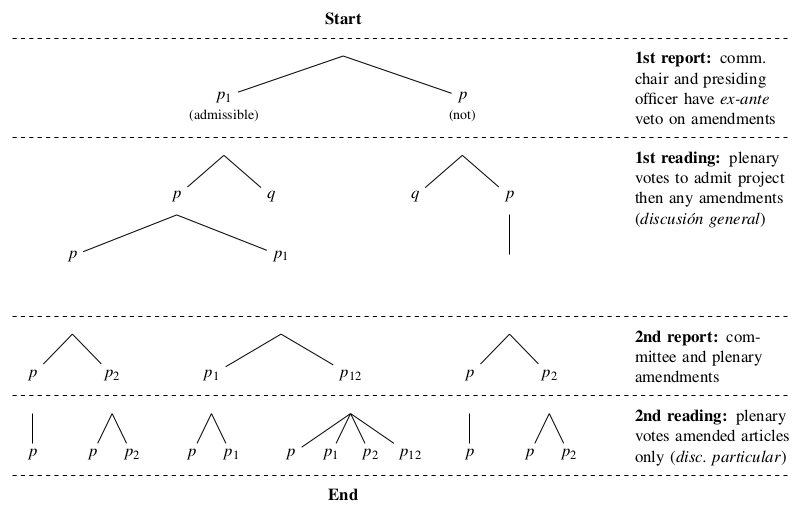
\includegraphics[width=\columnwidth]{../../graphs/chileAgendaBis.png} \\

    
}

%%%%%%%%%%%%%%%%%%%%%%%%%%%%%%%%%%%%%%%%%%%%%%%%%%%%%%%%%%%%%%%%%%%%%%%%%%%%%%%%%%%%%%%%%%%%%%%%
\frame {                      % SLIDE

    \frametitle{The urgency as a restrictive rule}

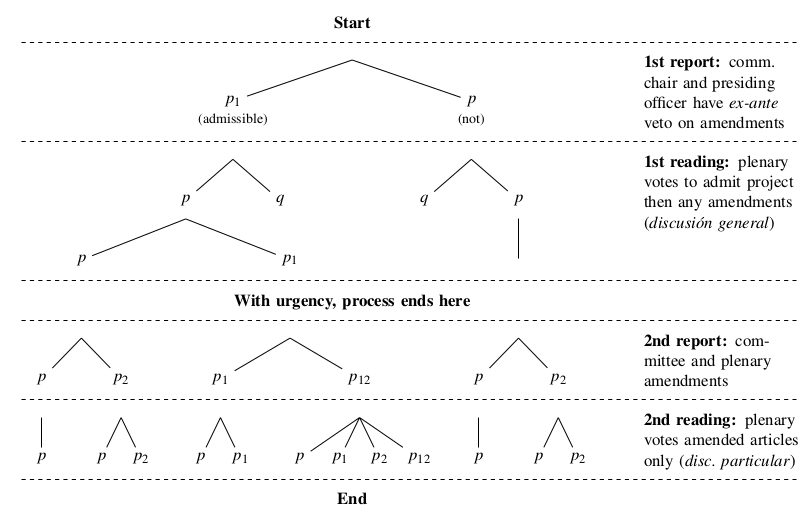
\includegraphics[width=\columnwidth]{../../graphs/chileAgenda.png} \\

    
}
%%%%%%%%%%%%%%%%%%%%%%%%%%%%%%%%%%%%%%%%%%%%%%%%%%%%%%%%%%%%%%%%%%%%%%%%%%%%%%%%%%%%%%%%%%%%%%%%
\frame {                      % SLIDE

    \frametitle{A game (extends Dion\&Huber 1996)}

    \begin{center}
      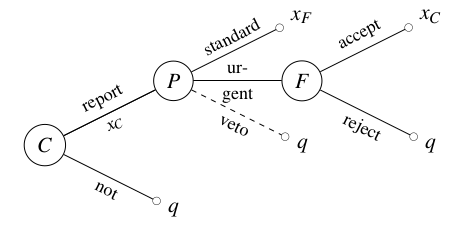
\includegraphics[width=.6\columnwidth]{../../graphs/game.png} \\
    \end{center}

\bi
\item Dotted branch = anticipation of a veto later on
\item Analysis with/without it (sustained/overridden veto)
\ei
}
%%%%%%%%%%%%%%%%%%%%%%%%%%%%%%%%%%%%%%%%%%%%%%%%%%%%%%%%%%%%%%%%%%%%%%%%%%%%%%%%%%%%%%%%%%%%%%%%
\frame {                      % SLIDE

    \frametitle{Analysis (spatial model)}

    \begin{center}
      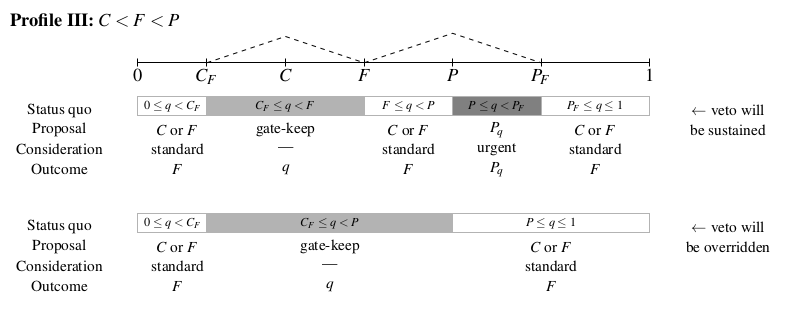
\includegraphics[width=\columnwidth]{../../graphs/prof3.png} \\
    \end{center}
}
%%%%%%%%%%%%%%%%%%%%%%%%%%%%%%%%%%%%%%%%%%%%%%%%%%%%%%%%%%%%%%%%%%%%%%%%%%%%%%%%%%%%%%%%%%%%%%%%
\frame {                      % SLIDE

    \frametitle{Analysis (spatial model)}

    \begin{center}
      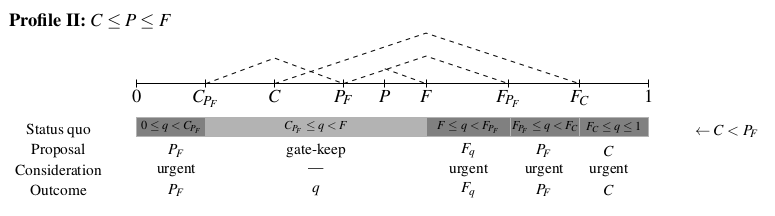
\includegraphics[width=\columnwidth]{../../graphs/prof2a.png} \\
    \end{center}
}
%%%%%%%%%%%%%%%%%%%%%%%%%%%%%%%%%%%%%%%%%%%%%%%%%%%%%%%%%%%%%%%%%%%%%%%%%%%%%%%%%%%%%%%%%%%%%%%%
\frame {
  \frametitle{Key result}
Standard consideration only when \\ \alert{president and committee on either side of the floor median}

\bigskip \pause

\begin{block}{Hypothesis 2: $Pr(\text{bill urgent})$}
  a.  up when president and committee chair \textbf{co-partisan} \\
  b.  up when committee chair from president's \textbf{coalition}
  \end{block}

}
%%%%%%%%%%%%%%%%%%%%%%%%%%%%%%%%%%%%%%%%%%%%%%%%%%%%%%%%%%%%%%%%%%%%%%%%%%%%%%%%%%%%%%%%%%%%%%%%
\frame {                      % SLIDE

    \frametitle{Data}

\bi
\item Original dataset of bill histories 1998--2014
%\item Many missing records before 1998 
%\item Covers 3+ presidencies, variance in president's status\\ 
%(coalition unity, Carey 2002, Alem�n\&Saiegh 2007)
\ei

\pause

\centering
\setbeamercovered{invisible} 
\begin{tabular}{lr}
Executive bills          &              \\ \hline
introduced               &       1,461  \onslide<3-> \\ \hdashline
passed                   &       1,059  \\
as \% introduced         &   \emph{72}  \onslide<4-> \\ \hdashline
declared urgent          &         834  \\
as \% introduced         &   \emph{57}  \onslide<5-> \\ \hdashline
declared urgent \& passed&         641  \\
as \% declared urgent    &   \emph{77}  \\ \hline
\end{tabular}

%% \centering
%% \setbeamercovered{invisible} 
%% \begin{tabular}{lrrr}
%%                          &  by           &  by          &    by      \\
%% Bills                    &  legislators  &  president   &    ~~~~either  \\ \hline
%% introduced               &        5,533  &       1,469  &     7,002  \\
%% as \%                    &    \emph{79}  &   \emph{21}  & \emph{100} \onslide<3-> \\ \hdashline
%% passed                   &          404  &       1,067  &     1,471  \\
%% as \%                    &    \emph{27}  &   \emph{73}  & \emph{100} \\
%% as \% introduced         &     \emph{7}  &   \emph{73}  &  \emph{21} \onslide<4-> \\ \hdashline
%% declared urgent          &          351  &       1,016  &     1,367  \\
%% as \%                    &    \emph{26}  &   \emph{74}  & \emph{100} \\
%% as \% introduced         &     \emph{6}  &   \emph{69}  &  \emph{20} \onslide<5-> \\ \hdashline
%% declared urgent \& passed&          167  &         762  &       929  \\
%% as \%                    &    \emph{18}  &   \emph{82}  & \emph{100} \\
%% as \% declared urgent    &    \emph{48}  &   \emph{75}  &  \emph{68} \\ \hline
%% \end{tabular}

}
%%%%%%%%%%%%%%%%%%%%%%%%%%%%%%%%%%%%%%%%%%%%%%%%%%%%%%%%%%%%%%%%%%%%%%%%%%%%%%%%%%%%%%%%%%%%%%%%
\frame {                      % SLIDE

  \frametitle{Multivariate model}

  \begin{center}
  $y = \begin{cases} 1 \text{ if bill urgent in C�mara}\\ 0 \text{ otherwise} \end{cases}$

  \bigskip

  $\text{logit}(y) = \alpha + \beta \text{Co-partisan chair} + \gamma \text{controls} + \text{error}$
  \end{center}
\bi
\item Co-partisan and coalition chair specifications
\item Prediction: \alert{$\beta >0$}
\item Controls include:
  \bi
  \item Multiple referrals
  \item Hacienda referral
  \item Introduced in Senate 
%  \item Senate majority
%  \item Relax deadlines
  \item Year remaining
%  \item Presidential approval    
  \ei
\item Fixed/mixed effects for verification
\ei
  
  }
%%%%%%%%%%%%%%%%%%%%%%%%%%%%%%%%%%%%%%%%%%%%%%%%%%%%%%%%%%%%%%%%%%%%%%%%%%%%%%%%%%%%%%%%%%%%%%%%
\frame {                      % SLIDE

    \frametitle{Logit regressions}

    \begin{center}
      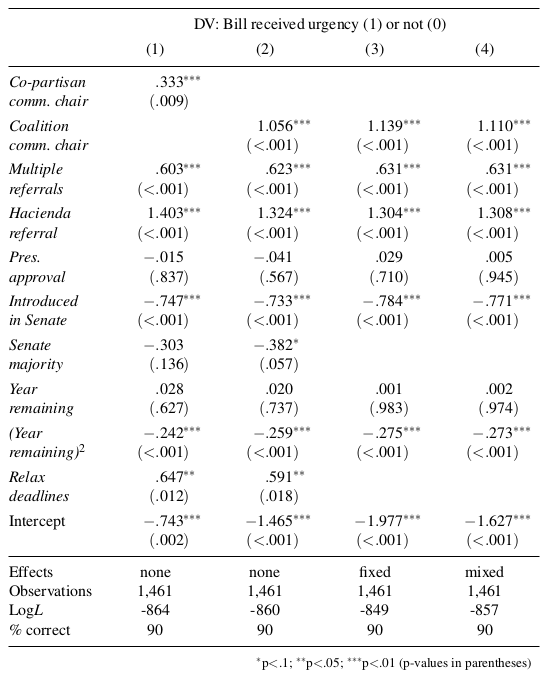
\includegraphics[width=.6\columnwidth]{../../graphs/logits.png} \\ 
    \end{center}
}
%%%%%%%%%%%%%%%%%%%%%%%%%%%%%%%%%%%%%%%%%%%%%%%%%%%%%%%%%%%%%%%%%%%%%%%%%%%%%%%%%%%%%%%%%%%%%%%%
\frame {                      % SLIDE

    \frametitle{Marginal effects (95\% confidence intervals)}

    \begin{center}
      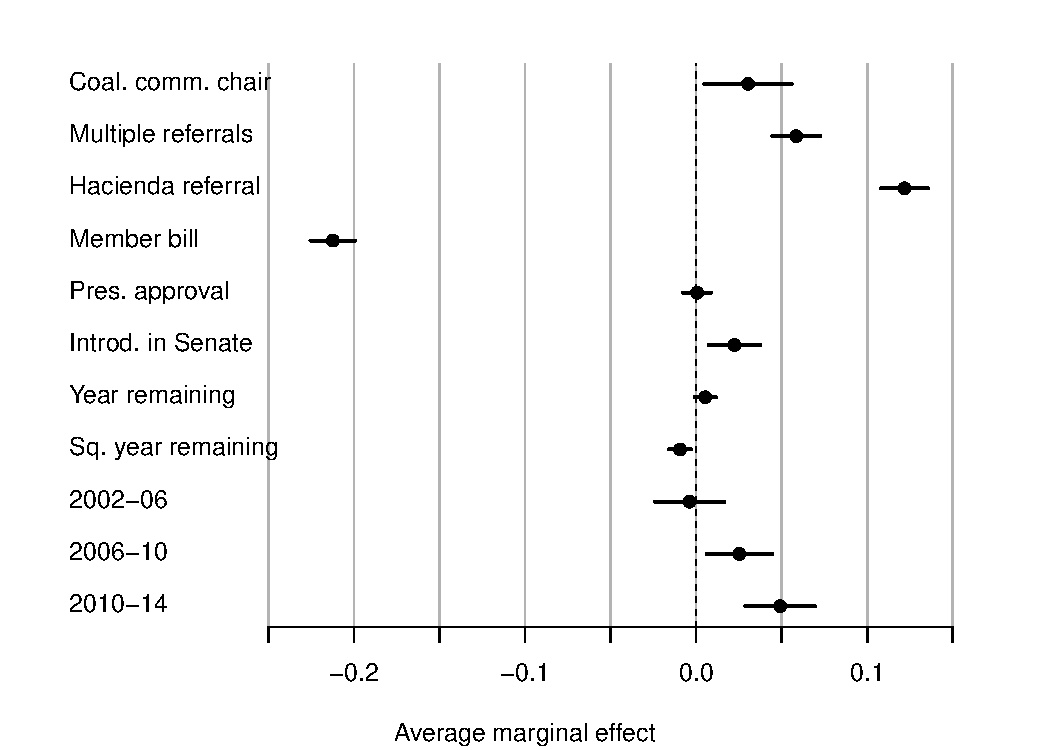
\includegraphics[width=.8\columnwidth]{../../graphs/avgMgEffects.pdf} \\
    \end{center}
}
%%%%%%%%%%%%%%%%%%%%%%%%%%%%%%%%%%%%%%%%%%%%%%%%%%%%%%%%%%%%%%%%%%%%%%%%%%%%%%%%%%%%%%%%%%%%%%%%
\frame {                      % SLIDE

    \frametitle{Predicted probability that bill is urgent}

    \begin{center}
      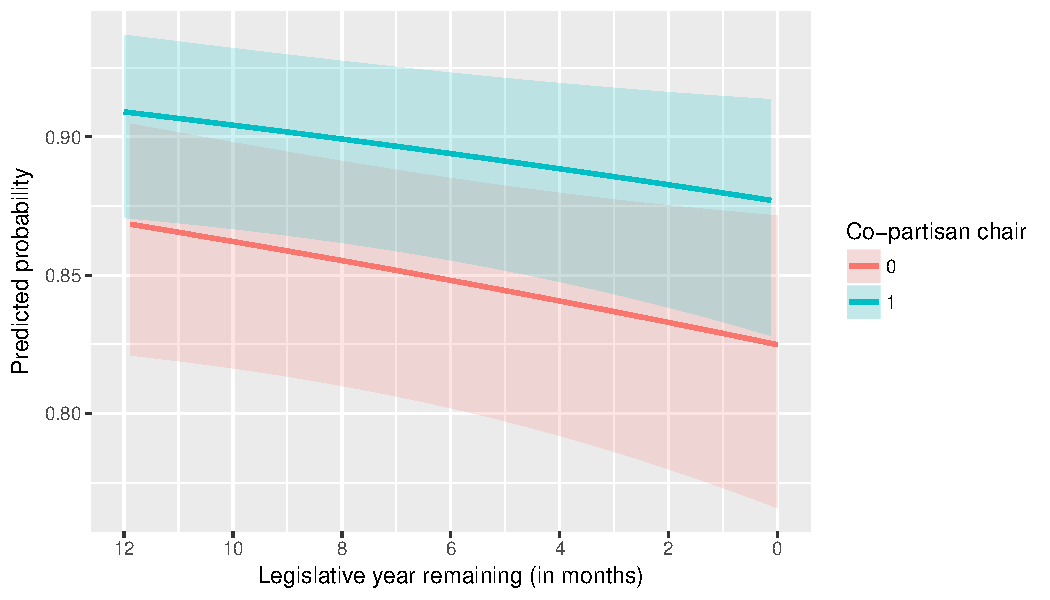
\includegraphics[width=\columnwidth]{../../graphs/predictedPr.pdf} \\
    \end{center}
}
%%%%%%%%%%%%%%%%%%%%%%%%%%%%%%%%%%%%%%%%%%%%%%%%%%%%%%%%%%%%%%%%%%%%%%%%%%%%%%%%%%%%%%%%%%%%%%%%
\frame {                      % SLIDE

    \frametitle{Urgency message types (incl.\ member bills)}

\centering

\resizebox{\linewidth}{!}{
\begin{tabular}{rrrrr|r}
      & 1998--2002 & 2002--2006 & 2006--2010 & 2010--2014 & 1998--2014 \\ \hline
 \textbf{Act now}             & \textbf{5}  & \textbf{6}  & \textbf{3}  & \textbf{4}  & \textbf{4} \\ 
 \textbf{2-week notice}       & \textbf{16} & \textbf{14} & \textbf{9}  & \textbf{23} & \textbf{16} \\ 
 4-week notice       & 29 & 22 & 13 & 12 & 17 \\ \hdashline
 Shorten deadline    & 2  & 2  & 2  & 4  &  3 \\ 
 Extend deadline     & 29 & 33 & 41 & 43 & 39 \\ \hdashline
 Withdraw (act now)  & 1  & 2  & 2  & 2  &  2 \\ 
 Withdraw (2-week)   & 7  & 10 & 14 & 8  & 10 \\ 
 Withdraw (4-week)   & 10 & 11 & 17 & 3  & 10 \\ \hline
 Total messages      & 100 & 100 & 100 & 100 & 100 \\ 
(N)                  & (1,268) & (1,881) & (4,941) & (5,643) & (13,733)\\ %\hline
% Senate status       & \emph{tied} & \emph{tied} & \emph{gov.} & \emph{opp.} & \\
\end{tabular}
}

}
%%%%%%%%%%%%%%%%%%%%%%%%%%%%%%%%%%%%%%%%%%%%%%%%%%%%%%%%%%%%%%%%%%%%%%%%%%%%%%%%%%%%%%%%%%%%%%%%
\frame {                      % SLIDE
    \frametitle{Wrap-up}

\bi
\item Urgency authority = closed rule
\item Unlike Rules Committee, Chilean prez controls this
\item Evidence that president--chair preference similarity $\rightarrow$ surge
\item More tests:
  \be
  \item Use nominate scores instead of partisan dummies
  \item Study amendments, admitted v.\ not: $Corr(\text{amendments, urgency})<0$?  
  \item Shorten deadlines $\rightarrow$ abort amendment threats?
  \ee
%\item 2/5 messages extend deadline, 1/5 withdraw urgency
  %% \be
  %% \item Which exec.\ proposals not urgent? 
  %% \item How do member proposals become urgent? Vote trading?
  %% \ee
\item Comments and critiques welcome
\ei

\pause

\center{\textbf{Thank you!}}

}
%%%%%%%%%%%%%%%%%%%%%%%%%%%%%%%%%%%%%%%%%%%%%%%%%%%%%%%%%%%%%%%%%%%%%%%%%%%%%%%%%%%%%%%%%%%%%%%%
\frame {                      % SLIDE
    \frametitle{D�nde dudo}
\be
\item Framing
\item Sacar m�s jugo del puzzle del presidente como \emph{Rules-maker}
\item Where to submit?
\ee

}
%%%%%%%%%%%%%%%%%%%%%%%%%%%%%%%%%%%%%%%%%%%%%%%%%%%%%%%%%%%%%%%%%%%%%%%%%%%%%%%%%
\frame[plain] {                      % SLIDE

%    \frametitle{}

\Large
\centering
\textbf{Extra material}
}
%%%%%%%%%%%%%%%%%%%%%%%%%%%%%%%%%%%%%%%%%%%%%%%%%%%%%%%%%%%%%%%%%%%%%%%%%%%%%%%%%%%%%%%%%%%%%%%%
%%%%%%%%%%%%%%%%%%%%%%%%%%%%%%%%%%%%%%%%%%%%%%%%%%%%%%%%%%%%%%%%%%%%%%%%%%%%%%%%%%%%%%%%%%%%%%%%
\frame {                      % SLIDE

    \frametitle{Original data}

\href{http://www.camara.cl/pley/pley_detalle.aspx?prmID=498&prmBL=2035-06}{\url{www.camara.cl}} very sharp \\
Scraped with \texttt{Python}'s Selenium library $\rightarrow$ \alert{bill histories 1990--2014}

\bigskip

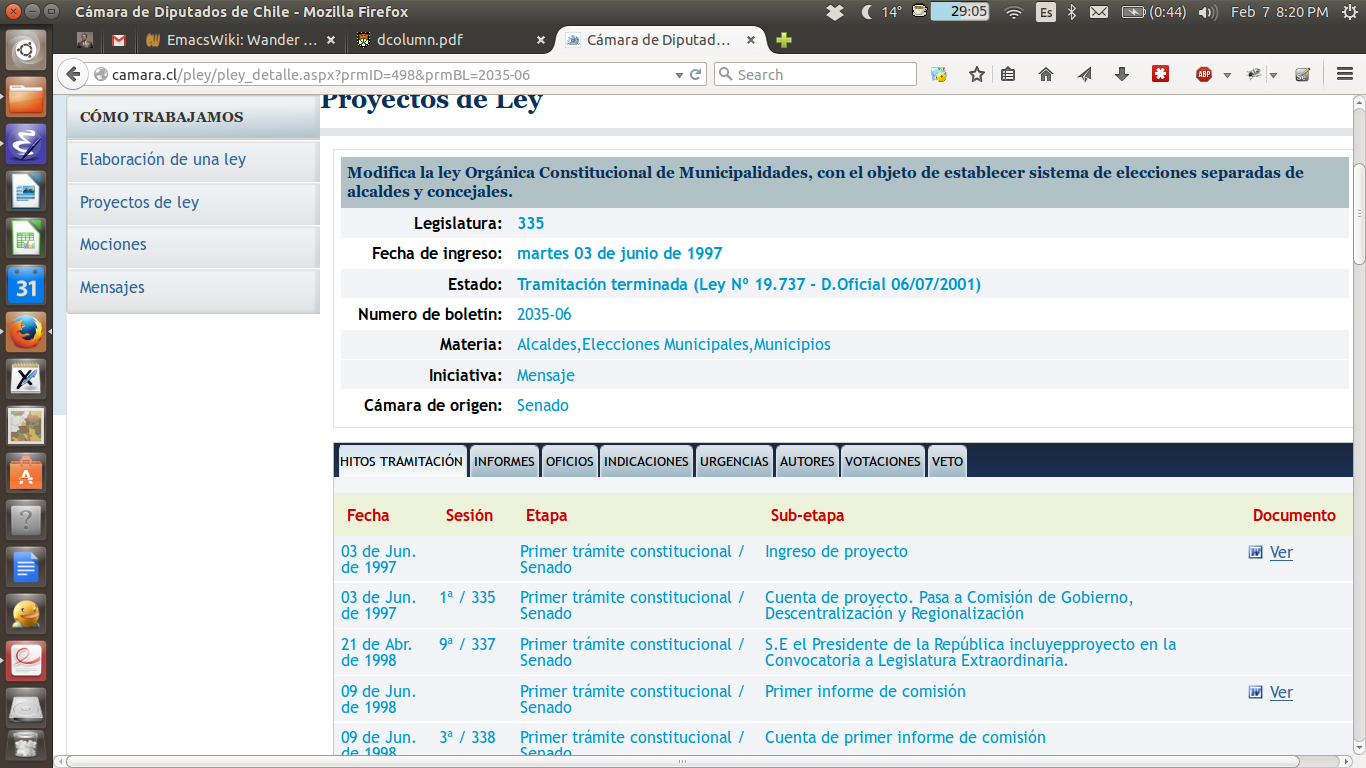
\includegraphics[width=\columnwidth]{../../graphs/hit.png} \\

}
%%%%%%%%%%%%%%%%%%%%%%%%%%%%%%%%%%%%%%%%%%%%%%%%%%%%%%%%%%%%%%%%%%%%%%%%%%%%%%%%%%%%%%%%%%%%%%%%
\frame {                      % SLIDE

    \frametitle{Original data}

\href{http://www.camara.cl/pley/pley_detalle.aspx?prmID=498&prmBL=2035-06}{\url{www.camara.cl}} very sharp \\
Scraped with \texttt{Python}'s Selenium library $\rightarrow$ \alert{bill histories 1990--2014}

\bigskip

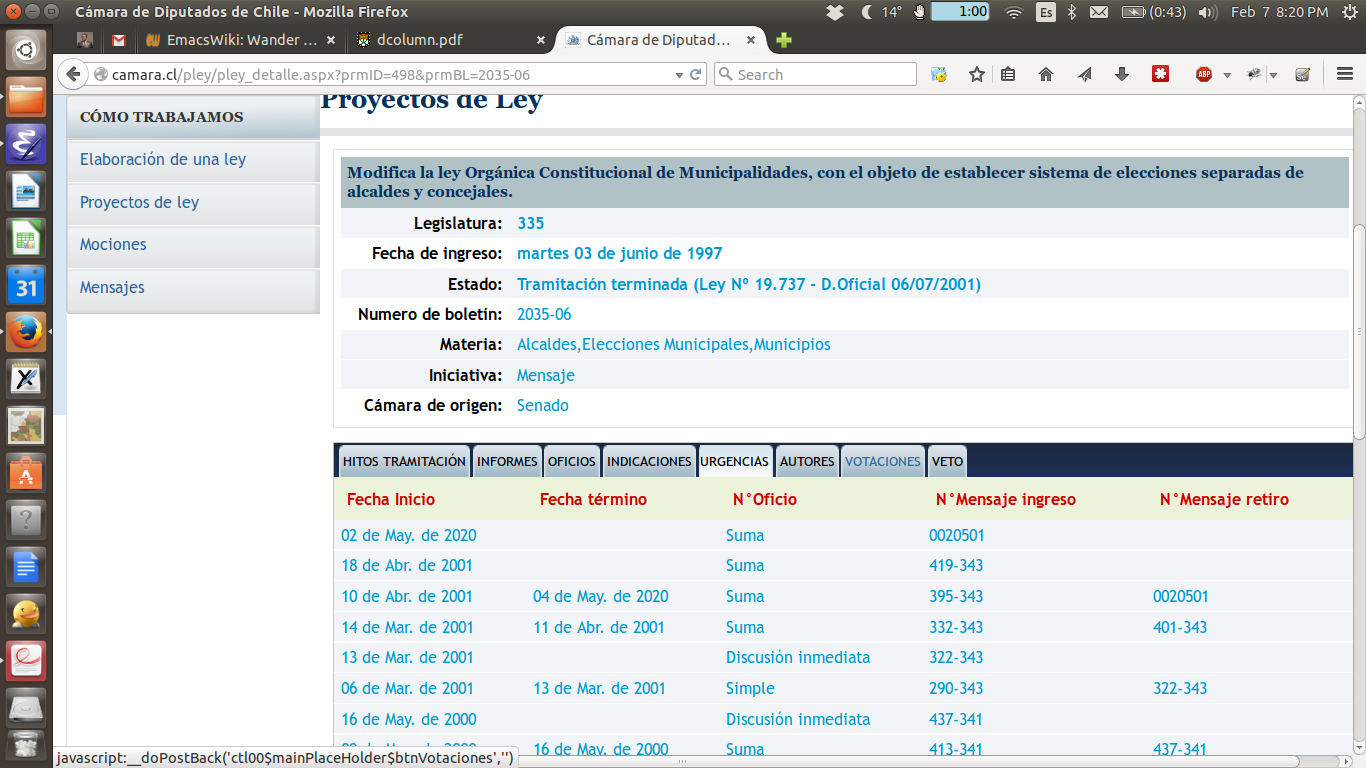
\includegraphics[width=\columnwidth]{../../graphs/urg.png} \\

}
%%%%%%%%%%%%%%%%%%%%%%%%%%%%%%%%%%%%%%%%%%%%%%%%%%%%%%%%%%%%%%%%%%%%%%%%%%%%%%%%%%%%%%%%%%%%%%%%
\frame {                      % SLIDE

    \frametitle{Partisan status of government}

\begin{center}
\begin{tabular}{lrrrr}
Coalition   & 1998--02    & 2002--06 & 2006--10 & 2010--14 \\ \hline
&\mc{4}{l}{\textbf{~~C\'amara de Diputados}} \\
President's & \color{green}{58}            & \color{green}{53}       & \color{green}{51}       & \color{YellowOrange}{50}       \\
Opposition  & 42            & 48       & 47       & 48       \\
Regional    &               &          & 3        & 2        \\ \hdashline
Total       & 100           & 100      & 100      & 100      \\ \hline
&\mc{4}{l}{\textbf{~~Senate}} \\
President's & \color{YellowOrange}{50} & \color{YellowOrange}{50}       & \color{green}{55}       & \color{red}{45}       \\
Opposition  & 50            & 50       & 45       & 55       \\ \hdashline
Total       & 100           & 100      & 100      & 100      \\ \hline
\end{tabular}
\end{center}

}
%%%%%%%%%%%%%%%%%%%%%%%%%%%%%%%%%%%%%%%%%%%%%%%%%%%%%%%%%%%%%%%%%%%%%%%%%%%%%%%%%%%%%%%%%%%%%%%%
\frame {                      % SLIDE

    \frametitle{Recidivism}
\begin{center}

\begin{tabular}{rr}
Number of & Bill  \\
messages  & freq.~\% \\ \hline
1        &  \emph{16}   \\
2        &  \emph{18}   \\
3        &  \emph{11}   \\
4        &  \emph{8}    \\
5--10    &  \emph{25}   \\
11--20   &  \emph{14}   \\
21--71   &  \emph{9}    \\ \hline
Total    & \emph{100}   \\ 
(N)      & (1,367)      \\
\end{tabular} 

\bigskip

Micro-managing presidents? Look @ message contents

\end{center}
}
%%%%%%%%%%%%%%%%%%%%%%%%%%%%%%%%%%%%%%%%%%%%%%%%%%%%%%%%%%%%%%%%%%%%%%%%%%%%%%%%%%%%%%%%%%%%%%%%
\frame {                      % SLIDE

    \frametitle{Urgency message incidence}


\begin{center}
Weekly messages in one legislative year \\ black = original urgency
    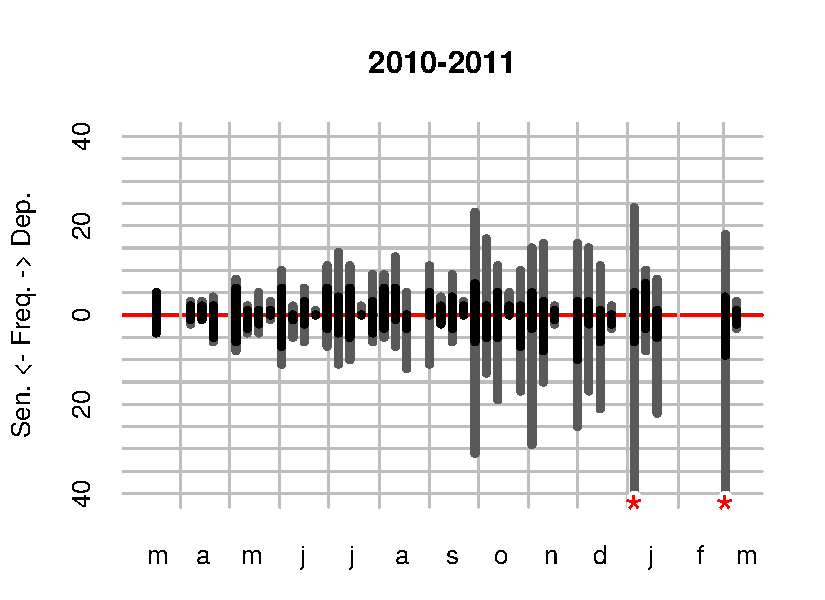
\includegraphics[width=.8\columnwidth]{../../graphs/urgenciasHistog2010.pdf} \\
(Two histograms: C\'amara above, Senate below \alert{zero} line)

\end{center}



}
%%%%%%%%%%%%%%%%%%%%%%%%%%%%%%%%%%%%%%%%%%%%%%%%%%%%%%%%%%%%%%%%%%%%%%%%%%%%%%%%%%%%%%%%%%%%%%%%
\frame {                      % SLIDE

    \frametitle{When all is urgent...}

\begin{center}
\begin{tabular}{cccc}
    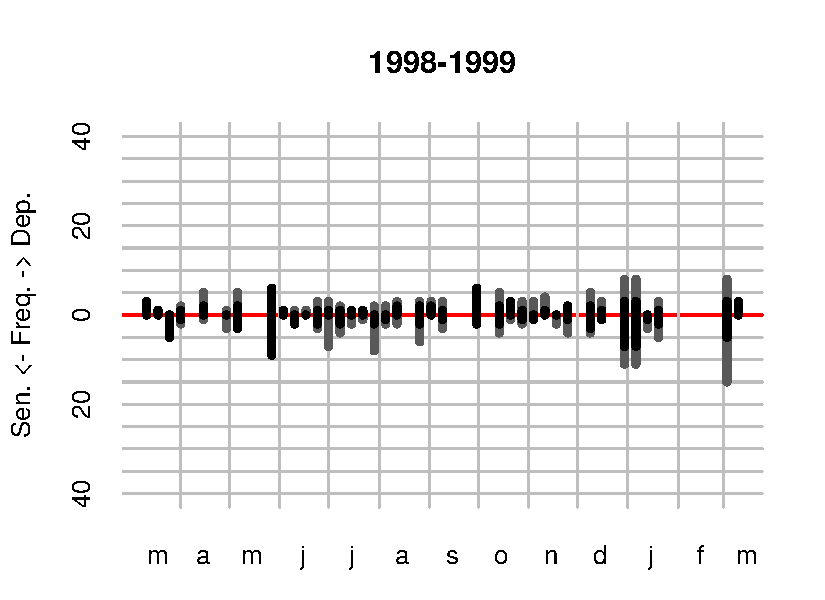
\includegraphics[width=.22\columnwidth]{../../graphs/urgenciasHistog1998.pdf} &
    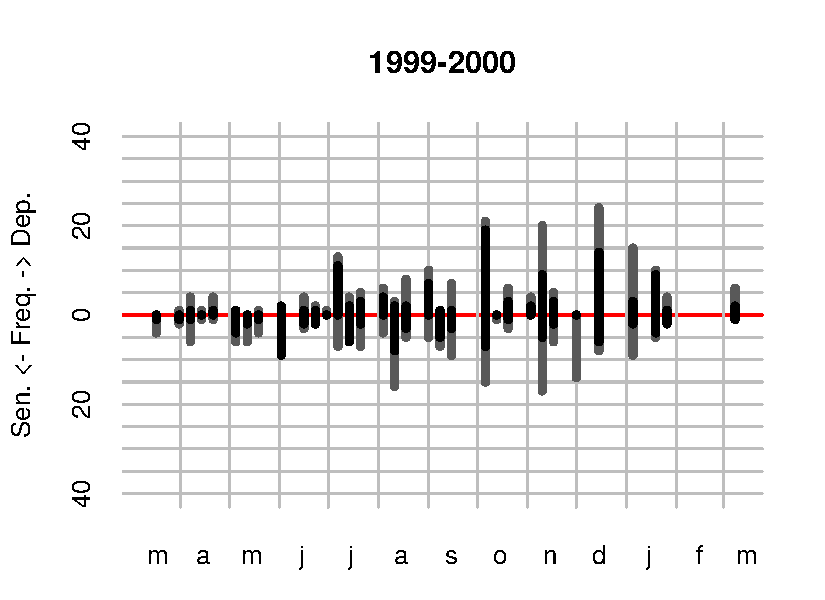
\includegraphics[width=.22\columnwidth]{../../graphs/urgenciasHistog1999.pdf} &
    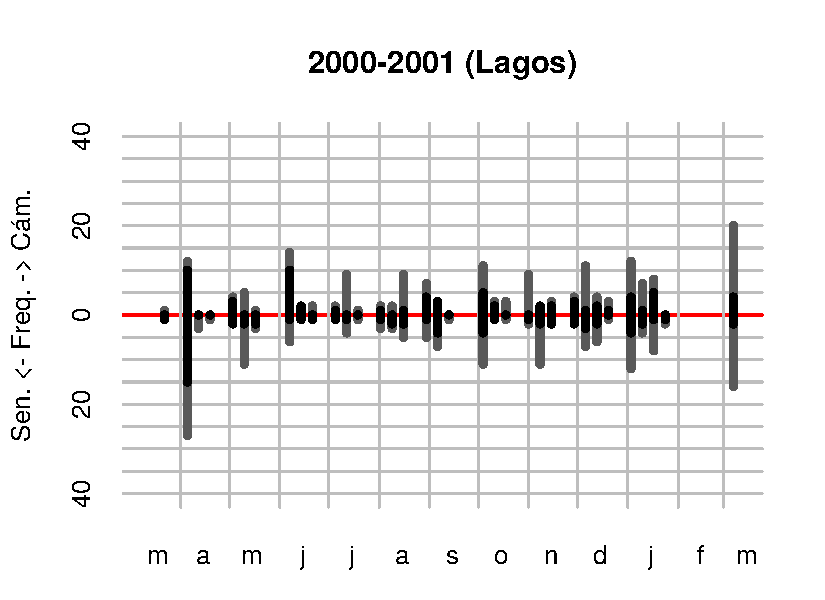
\includegraphics[width=.22\columnwidth]{../../graphs/urgenciasHistog2000.pdf} &
    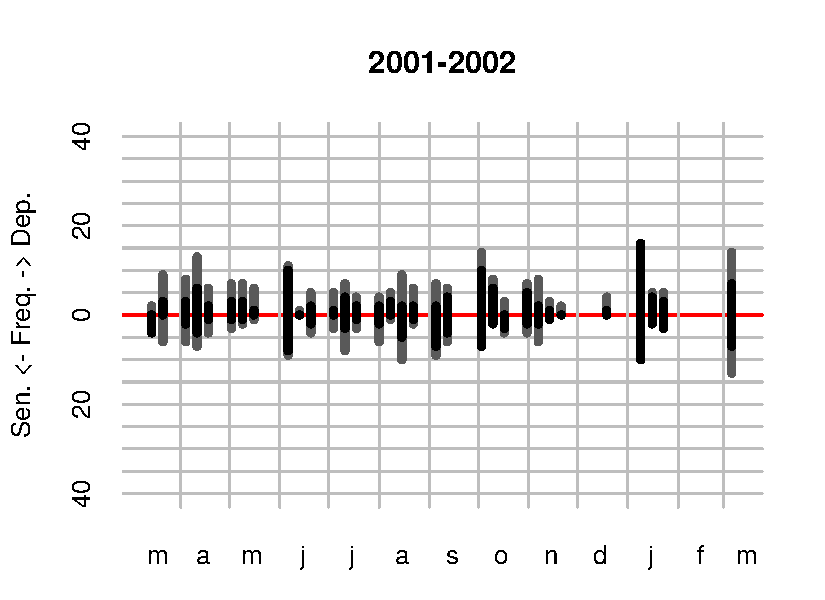
\includegraphics[width=.22\columnwidth]{../../graphs/urgenciasHistog2001.pdf} \\
    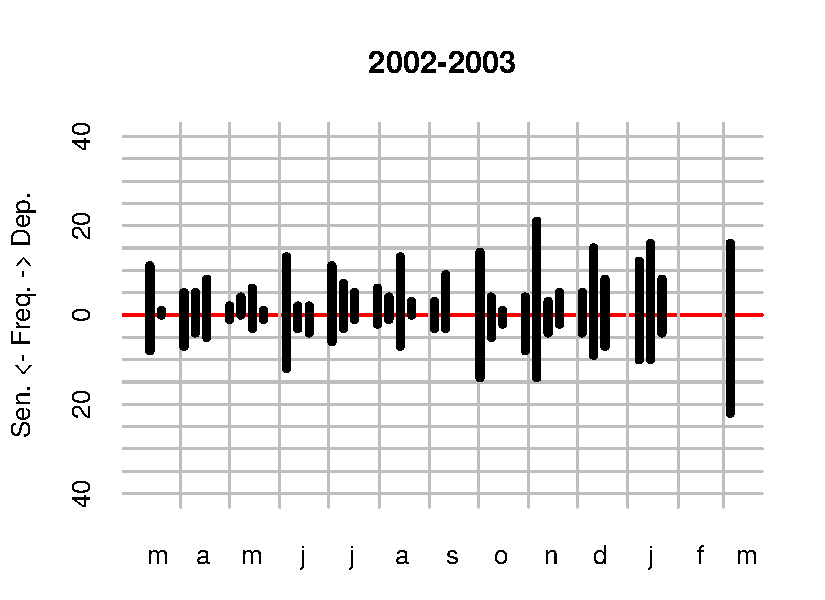
\includegraphics[width=.22\columnwidth]{../../graphs/urgenciasHistog2002.pdf} &
    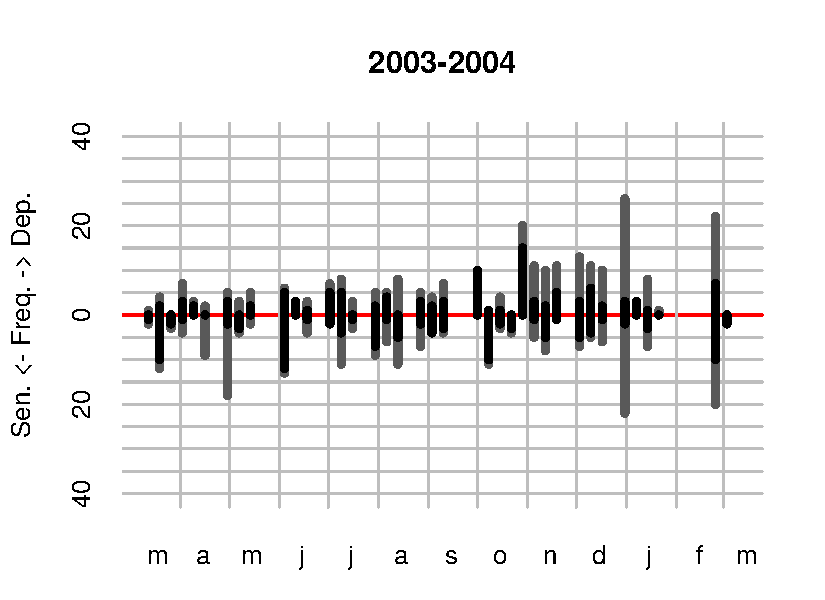
\includegraphics[width=.22\columnwidth]{../../graphs/urgenciasHistog2003.pdf} &
    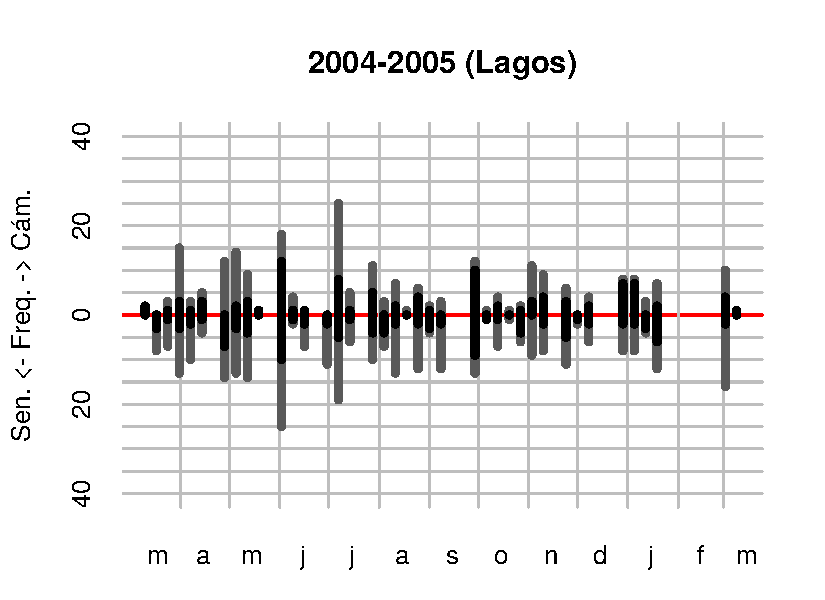
\includegraphics[width=.22\columnwidth]{../../graphs/urgenciasHistog2004.pdf} &
    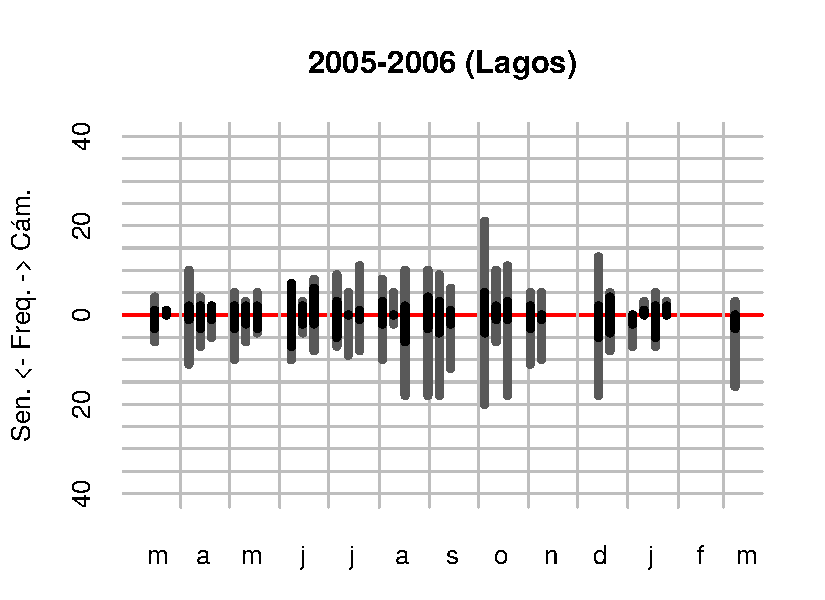
\includegraphics[width=.22\columnwidth]{../../graphs/urgenciasHistog2005.pdf} \\
    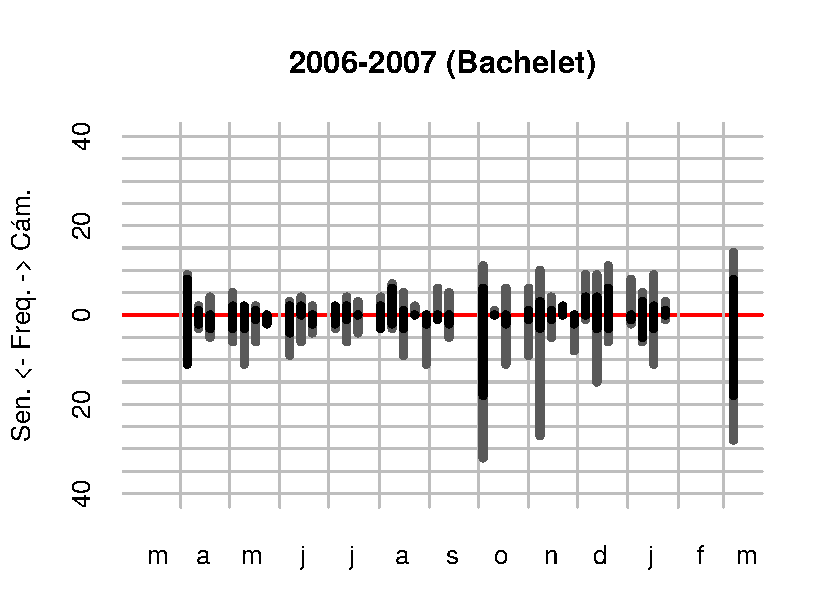
\includegraphics[width=.22\columnwidth]{../../graphs/urgenciasHistog2006.pdf} &
    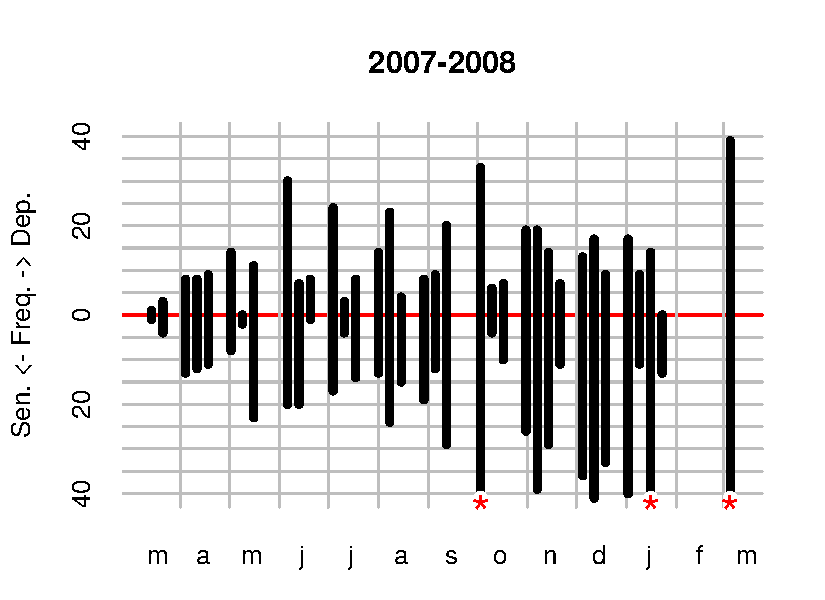
\includegraphics[width=.22\columnwidth]{../../graphs/urgenciasHistog2007.pdf} &
    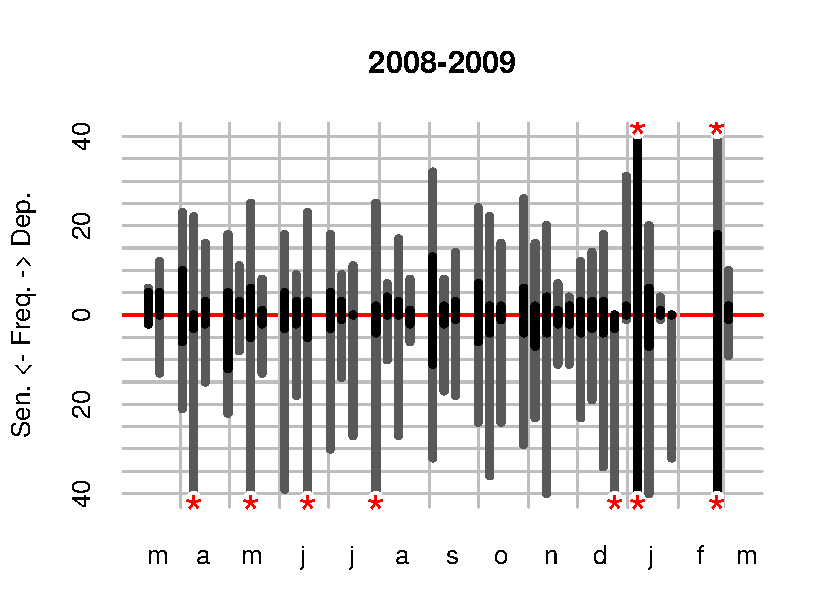
\includegraphics[width=.22\columnwidth]{../../graphs/urgenciasHistog2008.pdf} &
    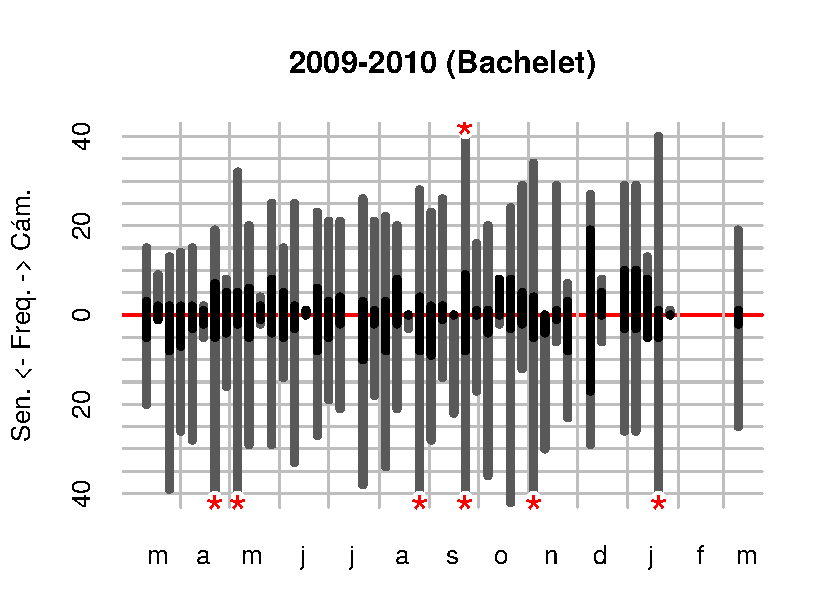
\includegraphics[width=.22\columnwidth]{../../graphs/urgenciasHistog2009.pdf} \\
    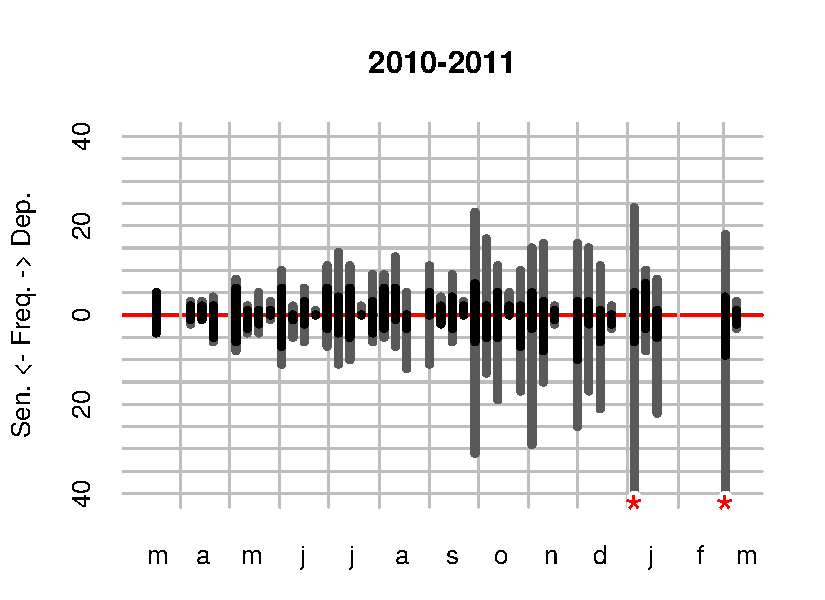
\includegraphics[width=.22\columnwidth]{../../graphs/urgenciasHistog2010.pdf} &
    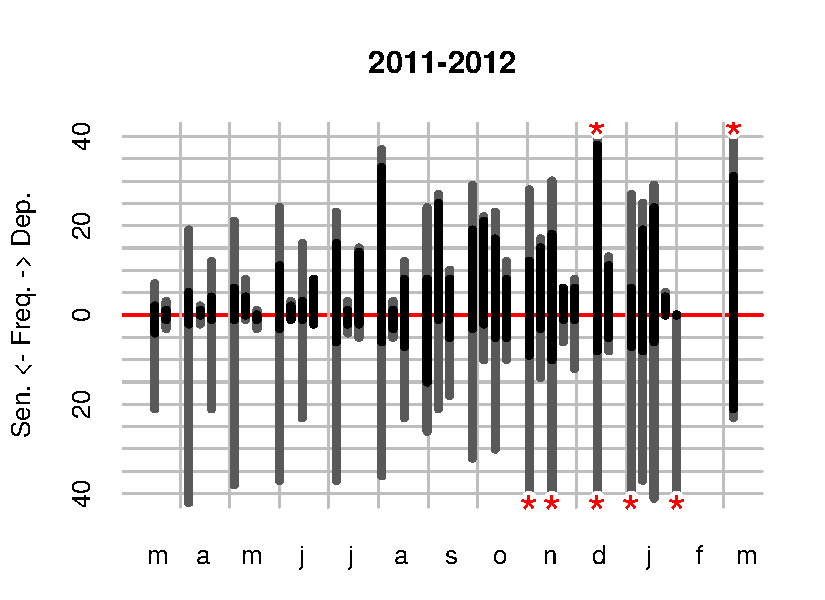
\includegraphics[width=.22\columnwidth]{../../graphs/urgenciasHistog2011.pdf} &
    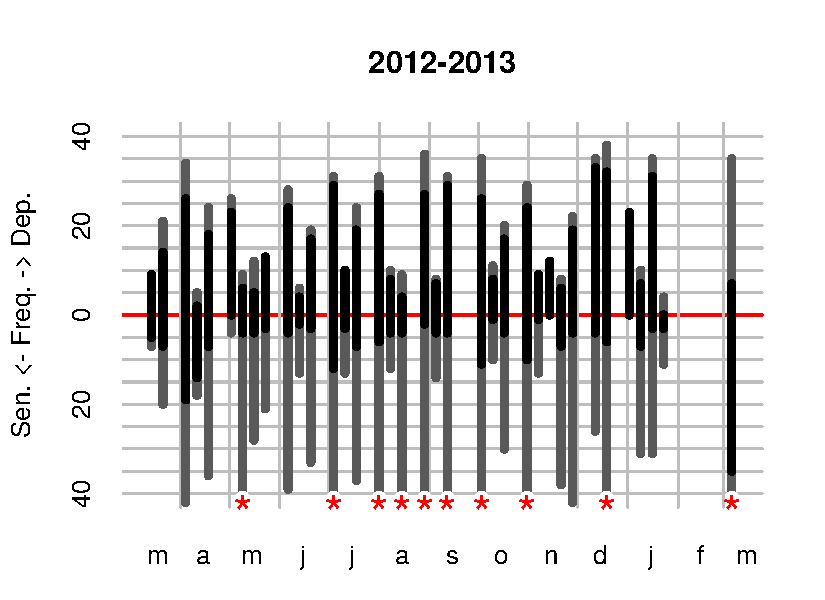
\includegraphics[width=.22\columnwidth]{../../graphs/urgenciasHistog2012.pdf} &
    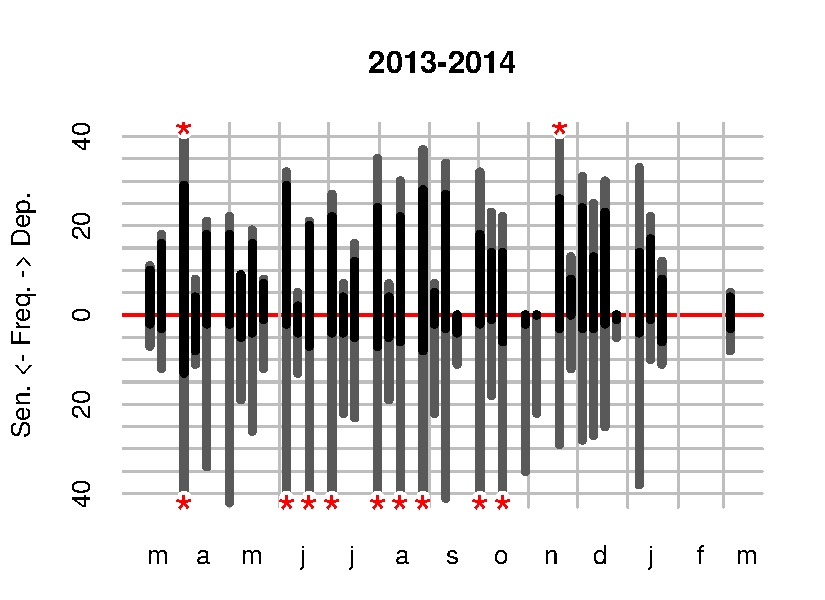
\includegraphics[width=.22\columnwidth]{../../graphs/urgenciasHistog2013.pdf} \\
\end{tabular}
\end{center}
}

%%%%%%%%%%%%%%%%%%%%%%%%%%%%%%%%%%%%%%%%%%%%%%%%%%%%%%%%%%%%%%%%%%%%%%%%%%%%%%%%%%%%%%%%%%%%%%%%
\frame {                      % SLIDE

    \frametitle{Lend a helping hand}


25\% urgencies were for member bills. Vote trading?


\begin{center}

\begin{tabular}{rrr}
                    &  \mc{2}{c}{Urgency by} \\
                    &  \mc{2}{c}{Concertaci�n president} \\
Concertaci�n sponsors            &  yes           & no          \\ \hline
all     &  \color{green}{\emph{39}}     & \color{red}{\emph{26}}   \\ 
some    &  \emph{40}     & \emph{48}   \\
none    &  \color{red}{\emph{21}}     & \color{green}{\emph{26}}   \\ \hline
        &  \emph{100}    & \emph{100}  \\
%(N)                 &      (230)     & (121)       \\
\end{tabular}
\end{center}
}


%%%%%%%%%%%%%%%%%%%%%%%%%%%%%%%%%%%%%%%%%%%%%%%%%%%%%%%%%%%%%%%%%%%%%%%%%%%%%%%%%%%%%%%%%%%%%%%%
\frame {                      % SLIDE

    \frametitle{Committee report after an urgency}

\begin{center}
\begin{tabular}{lr}
Message             &  Report w/i deadline (\%) \\ \hline
Act now             &  63     \\
2-week notice       &  27     \\
4-week notice       &  25     \\
Deadline shortened  &  41     \\
Deadline extended   &  23     \\
Withdrawn           &  6      \\ \hline
All                 &  27     \\
\end{tabular}
\end{center}


}
%%%%%%%%%%%%%%%%%%%%%%%%%%%%%%%%%%%%%%%%%%%%%%%%%%%%%%%%%%%%%%%%%%%%%%%%%%%%%%%%%%%%%%%%%%%%%%%%
\frame {                      % SLIDE

    \frametitle{Three event count models}

% \begin{tabular}{ccc|cc}
%       & \mc{2}{c}{DV} & \mc{2}{c}{IV} \\
%       & \mc{2}{c}{N reports of bills} & \mc{2}{c}{N urgencies on bills} \\
% Model & by           & by     & by     & referred to \\ \hline
% (a)   & Hacienda     & exec.  & exec.  & Hacienda    \\
% (b)   & Hacienda     & MC     & exec.  & Hacienda    \\
% (d)   & Hacienda     & MC     & MC     & Hacienda    \\
% (e)   & any comm.    & exec.  & exec.  & any         \\
% (f)   & any comm.    & MC     & exec.  & any         \\
% \end{tabular}

\begin{center} 

\begin{tabular}{c|c}
$e$ & $m$ \\
\begin{tikzpicture}[scale=.6]
\def\circleH{(0,1) circle (1cm)}
\def\circleU{(1,1) circle (1cm)}
\def\circleR{(.5,0) circle (1cm)}
\draw[gray] \circleH;
\draw[gray] \circleU;
\draw[gray] \circleR;
\begin{scope}
  \clip \circleH;
  \draw \circleU;
\end{scope}
\begin{scope}
  \clip \circleU;
  \draw \circleH;
\end{scope}
\node[gray] at (-1.25,1.25) {\footnotesize{$H$}};
\node[gray] at (2.25,1.25) {\footnotesize{$U$}};
\node[gray] at (-.7,-.7) {\footnotesize{$R$}};
\node at (.5,2.25) {\footnotesize{$u^e$}};
%\node at (.5,1.4) {\footnotesize{$\bar{r}_{e}$}};
\node at (.5,.55) {\footnotesize{$r^e$}};
\end{tikzpicture}
&
\begin{tikzpicture}[scale=.6]
\def\circleH{(0,1) circle (1cm)}
\def\circleU{(1,1) circle (1cm)}
\def\circleR{(.5,0) circle (1cm)}
\draw[gray] \circleH;
\draw[gray] \circleU;
\draw[gray] \circleR;
\begin{scope}
  \clip \circleH;
  \draw \circleU;
\end{scope}
\begin{scope}
  \clip \circleU;
  \draw \circleH;
\end{scope}
\node[gray] at (-1.25,1.25) {\footnotesize{$H$}};
\node[gray] at (2.25,1.25) {\footnotesize{$U$}};
\node[gray] at (-.7,-.7) {\footnotesize{$R$}};
\node at (.5,2.25) {\footnotesize{$u^m$}};
%\node at (.5,1.4) {\footnotesize{$\bar{r}_{e}$}};
\node at (.5,.55) {\footnotesize{$r^m$}};
\end{tikzpicture}
\end{tabular}

\bigskip \pause

\begin{tabular}{c|c|c|}
\mc{1}{c}{ }  & \mc{2}{c}{DepVar} \\
\mc{1}{c}{IndVar}  &   \mc{1}{c}{$r^e$}  &  \mc{1}{c}{$r^m$}  \\ \cline{2-3}
$u^e$ &  Mod.~1  & Mod.~2  \\ \cline{2-3}
$u^m$ &          & Mod.~3  \\ \cline{2-3}
\end{tabular}

\bigskip

Weekly counts: $r^e_t = \beta_0 + \beta_1 u^e_t + \beta_2 u^e_{t-1} + ... $

\bigskip

Negative binomial regression

\end{center}

}
%%%%%%%%%%%%%%%%%%%%%%%%%%%%%%%%%%%%%%%%%%%%%%%%%%%%%%%%%%%%%%%%%%%%%%%%%%%%%%%%%%%%%%%%%%%%%%%%
\frame {                      % SLIDE

    \frametitle{Message effects on Hacienda reports, C\'amara}

%\setbeamercovered{invisible} 
\resizebox{\linewidth}{!}{
\begin{tabular}{l|ccccc|ccccc}
 %                & \mc{10}{c}{Effect on committee reports ($t=0$ is current week)}                                      \\
%                 &   \mc{10}{c}{Dependent variable:} \\ 
%                 & \mc{5}{c}{Exec.~bill reports $r^e$}     & \mc{5}{c}{MC bill reports $r^m$}                      \\
                 & \mc{5}{c}{Weekly reports}     & \mc{5}{c}{Weekly reports}                      \\
Type             & $t=0$    & 1        & 2       & 3       & 4         & $t=0$    & 1          & 2         & 3          & 4          \\ \hline
%\mc{11}{l}{\emph{Urgency targets: exec.~bills referred to Hacienda committee}}                                                                \\
                 &               \mc{5}{c|}{$u^e \rightarrow r^e$}  &           \mc{5}{c}{$u^e \rightarrow r^m$}                         \\ 
Act Now          &   $++$   &  $+$     &   $--$  &         &           &          &  $++$      &           &            &            \\
2-week notice    &          &  $++$    &         &    $--$ &           &     $++$ &  $-$       &  $++$     &            &            \\
4-week notice    &          &          &         &    $++$ &      $++$ &          &            &           &            &            \\
Shorten deadline &          &  $++$    &         &         &           &          &            &           &            &            \\ \hdashline
%\mc{11}{l}{\emph{Urgency targets: MC~bills referred to Hacienda committee}}                                                                   \\
                 &           \mc{5}{c|}{$u^m \rightarrow r^e$}      &              \mc{5}{c}{$u^m \rightarrow r^m$}                     \\ 
Act Now          &          &          &         &         &           &     $++$ &  $++$      &           &            &            \\           
2-week notice    & & \mc{3}{c}{\footnotesize{(not estimated)}} &       &          &            &  $++$     &      $++$  &            \\           
4-week notice    &          &          &         &         &           &          &            &           &            &            \\           
Shorten deadline &          &          &         &         &           &          &            &           &            &            \\ %\hdashline
%\mc{11}{l}{\emph{Urgency targets: any exec.~bill}}                                                                                            \\
%                  &          \mc{5}{c}{5: $U^e \rightarrow R^e$}        &         \mc{5}{c}{6: $U^e \rightarrow R^m$}                 \\ 
% Act Now          &   $++$   &  $++$    &   $--$  &         &           &          &            &           &            &            \\
% 2-week notice    &          &  $+$     &   $++$  &         &           &     $+$  &            &           &            &      $--$  \\
% 4-week notice    &          &          &         &         &           &          &            &           &            &      $++$  \\
% Shorten deadline &          &          &         &         &           &          &            &           &            &            \\ 
\hline
%\mc{11}{l}{\footnotesize{$++,--: p<.05$; $+,-: p<.1$ (one-tailed tests)}}                                                             \\
\end{tabular}
}

}
%%%%%%%%%%%%%%%%%%%%%%%%%%%%%%%%%%%%%%%%%%%%%%%%%%%%%%%%%%%%%%%%%%%%%%%%%%%%%%%%%%%%%%%%%%%%%%%%
\frame {                      % SLIDE

    \frametitle{Sequence: Pi�era bills}

\begin{tabular}{cc}
\textbf{Sent to Senate} & \textbf{Sent to C\'amara}\\
 ($N=90$) & ($N=314$) \\

\tikzstyle{mid}=[circle,draw]
\tikzstyle{middot}=[circle,draw,dashed]
\tiny
\begin{tikzpicture}[shorten >=1pt,node distance=2cm,auto,scale=.27]
\node at (-5,6) (st) {\footnotesize{\textbf{\texttt{start}}}};
\node[mid]       at (0,0)   (p)  {\textbf{Exec.}};
\node[mid,red]   at (0,6)   (n1) {\textbf{Sen.}};
\node[mid,green] at (6,0)   (n2) {\textbf{C\'am.}};
\node[mid,red]   at (0,-6)  (n3) {\textbf{Sen.}};
\node[mid]       at (-6,0)  (c)  {\textbf{Conf.}};
%\node[middot]    at (2,3)   (u)  {$u$};
%\node[middot]    at (3,-2)  (v)  {$u$};
%\node[middot]    at (-2,-3) (w)  {$u$};
%\node[middot]    at (-3,2)  (x)  {$u$};
\draw [-stealth] (st)                    edge node {100} (n1);
\draw [-stealth] (n1) [loop above]       edge node              {39} ();    % l11 $A$
%\draw [-stealth] (n1) [bend left,dashed] edge node              {79} (u);   % l1u $B$
\draw [-stealth] (n1) [out=0,in=90]      edge node              {61} (n2);  % l12 $C$
%\draw [-stealth] (u)  [bend left]        edge node              {31} (n1);  % lu1 $D$
%\draw [-stealth] (u)                     edge node              {48} (n2);  % lu2 $E$
\draw [-stealth] (n2) [loop right]       edge node              { 7} ();    % l22 $F$
\draw [-stealth] (n2) [out=-90,in=0]     edge node              {29} (n3);  % l23 $G$
%\draw [-stealth] (n2) [bend left,dashed] edge node              {47} (v);   % l2v $H$
\draw [-stealth] (n2) [out=170, in=10]   edge node [swap]       {26} (p);   % l2p $I$
%\draw [-stealth] (v)  [bend left]        edge node              { 6} (n2);  % lv2 $J$
%\draw [-stealth] (v)                     edge node [swap]       {18} (p)    % lvp $K$
%                 (v)                     edge node              {23} (n3);  % lv3 $L$
\draw [-stealth] (n3) [loop below]       edge node              { 0} ();    % l33 $N$
\draw [-stealth] (n3) [out=180,in=-90]   edge node              {11} (c);   % l3c $O$
%\draw [-stealth] (n3) [bend left,dashed] edge node              {18} (w);   % l3w $P$
\draw [-stealth] (n3) [out=80, in=-80]   edge node [swap]       {18} (p);   % l3p $Q$
%\draw [-stealth] (w)  [bend left]        edge node [near start] { 0} (n3);  % lw3 $R$
%\draw [-stealth] (w)                     edge node              {11} (p)    % lwp $S$
%                 (w)                     edge node              { 7} (c);   % lwc $U$
\draw [-stealth] (c)  [loop left]        edge node              { 2} ();    % lcc $V$
%\draw [-stealth] (c)  [bend left,dashed] edge node              { 8} (x);   % lcx $W$
\draw [-stealth] (c)  [out=-10, in=-170] edge node [swap]       { 9} (p);   % lcp $X$
%\draw [-stealth] (x)  [bend left]        edge node              { 1} (c);   % lxc $Y$
%\draw [-stealth] (x)                     edge node              { 7} (p);   % lcp $Z$
\end{tikzpicture}

&

\tikzstyle{mid}=[circle,draw]
\tikzstyle{middot}=[circle,draw,dashed]
\tiny
\begin{tikzpicture}[shorten >=1pt,node distance=2cm,auto,scale=.27]
%\draw[help lines] (-6,-6) grid (6,6);
\node at (-5,6) (st) {\footnotesize{\textbf{\texttt{start}}}};
\node[mid]     at (0,0)   (p)  {\textbf{Exec.}};
\node[mid,green] at (0,6)   (n1) {\textbf{C\'am.}};
\node[mid,red]   at (6,0)   (n2) {\textbf{Sen.}};
\node[mid,green] at (0,-6)  (n3) {\textbf{C\'am.}};
\node[mid]       at (-6,0)  (c)  {\textbf{Conf.}};
%\node[middot]    at (2,3)   (u)  {$u$};
%\node[middot]    at (3,-2)  (v)  {$u$};
%\node[middot]    at (-2,-3) (w)  {$u$};
%\node[middot]    at (-3,2)  (x)  {$u$};
\draw [-stealth] (st)                    edge node {100} (n1);
\draw [-stealth] (n1) [loop above]       edge node              {22} ();    % l11 $A$
%\draw [-stealth] (n1) [bend left,dashed] edge node              {75} (u);   % l1u $B$
\draw [-stealth] (n1) [out=0,in=90]      edge node              {78} (n2);  % l12 $C$
%\draw [-stealth] (u)  [bend left]        edge node              {14} (n1);  % lu1 $D$
%\draw [-stealth] (u)                     edge node              {61} (n2);  % lu2 $E$
\draw [-stealth] (n2) [loop right]       edge node              {10} ();    % l22 $F$
\draw [-stealth] (n2) [out=-90,in=0]     edge node              {31} (n3);  % l23 $G$
%\draw [-stealth] (n2) [bend left,dashed] edge node              {57} (v);   % l2v $H$
\draw [-stealth] (n2) [out=170, in=10]   edge node [swap]       {36} (p);   % l2p $I$
%\draw [-stealth] (v)  [bend left]        edge node              { 7} (n2);  % lv2 $J$
%\draw [-stealth] (v)                     edge node [swap]       {24} (p)    % lvp $K$
%                 (v)                     edge node              {25} (n3);  % lv3 $L$
\draw [-stealth] (n3) [loop below]       edge node              { 0} ();    % l33 $N$
\draw [-stealth] (n3) [out=180,in=-90]   edge node              { 7} (c);   % l3c $O$
%\draw [-stealth] (n3) [bend left,dashed] edge node              {11} (w);   % l3w $P$
\draw [-stealth] (n3) [out=80, in=-80]   edge node [swap]       {24} (p);   % l3p $Q$
%\draw [-stealth] (w)  [bend left]        edge node [near start] { 0} (n3);  % lw3 $R$
%\draw [-stealth] (w)                     edge node              { 9} (p)    % lwp $S$
%                 (w)                     edge node              { 1} (c);   % lwc $U$
\draw [-stealth] (c)  [loop left]        edge node              { 0} ();    % lcc $V$
%\draw [-stealth] (c)  [bend left,dashed] edge node              { 5} (x);   % lcx $W$
\draw [-stealth] (c)  [out=-10, in=-170] edge node [swap]       { 7} (p);   % lcp $X$
%\draw [-stealth] (x)  [bend left]        edge node              { 0} (c);   % lxc $Y$
%\draw [-stealth] (x)                     edge node              { 5} (p);   % lcp $Z$
\end{tikzpicture}

\end{tabular}

}
%%%%%%%%%%%%%%%%%%%%%%%%%%%%%%%%%%%%%%%%%%%%%%%%%%%%%%%%%%%%%%%%%%%%%%%%%%%%%%%%%%%%%%%%%%%%%%%%
\frame {                      % SLIDE

    \frametitle{Sequence: Pi�era bills}

\begin{tabular}{cc}
\textbf{Sent to Senate} & \textbf{Sent to C\'amara}\\
 ($N=90$) & ($N=314$) \\

\tikzstyle{mid}=[circle,draw]
\tikzstyle{middot}=[circle,draw,dashed]
\tiny
\begin{tikzpicture}[shorten >=1pt,node distance=2cm,auto,scale=.27]
%\draw[help lines] (-6,-6) grid (6,6);
\node at (-5,6) (st) {\footnotesize{\textbf{\texttt{start}}}};
\node[mid]       at (0,0)   (p)  {\textbf{Exec.}};
\node[mid,red]   at (0,6)   (n1) {\textbf{Sen.}};
\node[mid,green] at (6,0)   (n2) {\textbf{C\'am.}};
\node[mid,red]   at (0,-6)  (n3) {\textbf{Sen.}};
\node[mid]       at (-6,0)  (c)  {\textbf{Conf.}};
\node[middot]    at (2,3)   (u)  {$u$};
\node[middot]    at (3,-2)  (v)  {$u$};
\node[middot]    at (-2,-3) (w)  {$u$};
\node[middot]    at (-3,2)  (x)  {$u$};
\draw [-stealth] (st)                    edge node {100} (n1);
\draw [-stealth] (n1) [loop above]       edge node              { 8} ();    % l11 $A$
\draw [-stealth] (n1) [bend left,dashed] edge node              {79} (u);   % l1u $B$
\draw [-stealth] (n1) [out=0,in=90]      edge node              {13} (n2);  % l12 $C$
\draw [-stealth] (u)  [bend left]        edge node              {31} (n1);  % lu1 $D$
\draw [-stealth] (u)                     edge node              {48} (n2);  % lu2 $E$
\draw [-stealth] (n2) [loop right]       edge node              { 1} ();    % l22 $F$
\draw [-stealth] (n2) [out=-90,in=0]     edge node              { 6} (n3);  % l23 $G$
\draw [-stealth] (n2) [bend left,dashed] edge node              {47} (v);   % l2v $H$
\draw [-stealth] (n2) [out=170, in=10]   edge node [swap]       { 8} (p);   % l2p $I$
\draw [-stealth] (v)  [bend left]        edge node              { 6} (n2);  % lv2 $J$
\draw [-stealth] (v)                     edge node [swap]       {18} (p)    % lvp $K$
                 (v)                     edge node              {23} (n3);  % lv3 $L$
\draw [-stealth] (n3) [loop below]       edge node              { 0} ();    % l33 $N$
\draw [-stealth] (n3) [out=180,in=-90]   edge node              { 4} (c);   % l3c $O$
\draw [-stealth] (n3) [bend left,dashed] edge node              {18} (w);   % l3w $P$
\draw [-stealth] (n3) [out=80, in=-80]   edge node [swap]       { 7} (p);   % l3p $Q$
\draw [-stealth] (w)  [bend left]        edge node [near start] { 0} (n3);  % lw3 $R$
\draw [-stealth] (w)                     edge node              {11} (p)    % lwp $S$
                 (w)                     edge node              { 7} (c);   % lwc $U$
\draw [-stealth] (c)  [loop left]        edge node              { 1} ();    % lcc $V$
\draw [-stealth] (c)  [bend left,dashed] edge node              { 8} (x);   % lcx $W$
\draw [-stealth] (c)  [out=-10, in=-170] edge node [swap]       { 2} (p);   % lcp $X$
\draw [-stealth] (x)  [bend left]        edge node              { 1} (c);   % lxc $Y$
\draw [-stealth] (x)                     edge node              { 7} (p);   % lcp $Z$
\end{tikzpicture}

&

\tikzstyle{mid}=[circle,draw]
\tikzstyle{middot}=[circle,draw,dashed]
\tiny
\begin{tikzpicture}[shorten >=1pt,node distance=2cm,auto,scale=.27]
%\draw[help lines] (-6,-6) grid (6,6);
\node at (-5,6) (st) {\footnotesize{\textbf{\texttt{start}}}};
\node[mid]     at (0,0)   (p)  {\textbf{Exec.}};
\node[mid,green] at (0,6)   (n1) {\textbf{C\'am.}};
\node[mid,red]   at (6,0)   (n2) {\textbf{Sen.}};
\node[mid,green] at (0,-6)  (n3) {\textbf{C\'am.}};
\node[mid]       at (-6,0)  (c)  {\textbf{Conf.}};
\node[middot]    at (2,3)   (u)  {$u$};
\node[middot]    at (3,-2)  (v)  {$u$};
\node[middot]    at (-2,-3) (w)  {$u$};
\node[middot]    at (-3,2)  (x)  {$u$};
\draw [-stealth] (st)                    edge node {100} (n1);
\draw [-stealth] (n1) [loop above]       edge node              { 8} ();    % l11 $A$
\draw [-stealth] (n1) [bend left,dashed] edge node              {75} (u);   % l1u $B$
\draw [-stealth] (n1) [out=0,in=90]      edge node              {17} (n2);  % l12 $C$
\draw [-stealth] (u)  [bend left]        edge node              {14} (n1);  % lu1 $D$
\draw [-stealth] (u)                     edge node              {61} (n2);  % lu2 $E$
\draw [-stealth] (n2) [loop right]       edge node              { 3} ();    % l22 $F$
\draw [-stealth] (n2) [out=-90,in=0]     edge node              { 6} (n3);  % l23 $G$
\draw [-stealth] (n2) [bend left,dashed] edge node              {57} (v);   % l2v $H$
\draw [-stealth] (n2) [out=170, in=10]   edge node [swap]       {12} (p);   % l2p $I$
\draw [-stealth] (v)  [bend left]        edge node              { 7} (n2);  % lv2 $J$
\draw [-stealth] (v)                     edge node [swap]       {24} (p)    % lvp $K$
                 (v)                     edge node              {25} (n3);  % lv3 $L$
\draw [-stealth] (n3) [loop below]       edge node              { 0} ();    % l33 $N$
\draw [-stealth] (n3) [out=180,in=-90]   edge node              { 6} (c);   % l3c $O$
\draw [-stealth] (n3) [bend left,dashed] edge node              {11} (w);   % l3w $P$
\draw [-stealth] (n3) [out=80, in=-80]   edge node [swap]       {15} (p);   % l3p $Q$
\draw [-stealth] (w)  [bend left]        edge node [near start] { 0} (n3);  % lw3 $R$
\draw [-stealth] (w)                     edge node              { 9} (p)    % lwp $S$
                 (w)                     edge node              { 1} (c);   % lwc $U$
\draw [-stealth] (c)  [loop left]        edge node              { 0} ();    % lcc $V$
\draw [-stealth] (c)  [bend left,dashed] edge node              { 5} (x);   % lcx $W$
\draw [-stealth] (c)  [out=-10, in=-170] edge node [swap]       { 2} (p);   % lcp $X$
\draw [-stealth] (x)  [bend left]        edge node              { 0} (c);   % lxc $Y$
\draw [-stealth] (x)                     edge node              { 5} (p);   % lcp $Z$
\end{tikzpicture}

\end{tabular}

}
%%%%%%%%%%%%%%%%%%%%%%%%%%%%%%%%%%%%%%%%%%%%%%%%%%%%%%%%%%%%%%%%%%%%%%%%%%%%%%%%%%%%%%%%%%%%%%%%
\section{Where next?}
%%%%%%%%%%%%%%%%%%%%%%%%%%%%%%%%%%%%%%%%%%%%%%%%%%%%%%%%%%%%%%%%%%%%%%%%%%%%%%%%%%%%%%%%%%%%%%%%
\frame {                      % SLIDE

    \frametitle{Two intuitions}

\begin{center}
schedule now $\neq$ passage \\ certainly, but
\end{center}

\bigskip

\be
\item Imperfect negative agenda control
  \bi
  \item Committee gatekeeking $\rightarrow$ silent death \\ (Weingast\&Marshall 1988)
  \item Could majority cartel operate? Must include president \\ (Cox\&McCubbins 2005)
  \ei
\item Dilatory tactics
  \bi
  \item Worsen legislative bottleneck (Cox 1987)
  \item Exploit impatience of those next in line \\ (Wawro\&Schickler 2007)
  \ei
\ee

}
%%%%%%%%%%%%%%%%%%%%%%%%%%%%%%%%%%%%%%%%%%%%%%%%%%%%%%%%%%%%%%%%%%%%%%%%%%%%%%%%%%%%%%%%%%%%%%%%

\end{document}
%%%%%%%%%%%%%%%%%%%%%%%%%%%%%%%%%%%%%%%%%%%%%%%%%%%%%%%%%%%%%%%%%%%%%%%%%%%%%%%%%%%%%%%%%%%%%%%% 
\frame {                      % SLIDE

    \frametitle{Daily messages 1998--99}

\begin{center}
    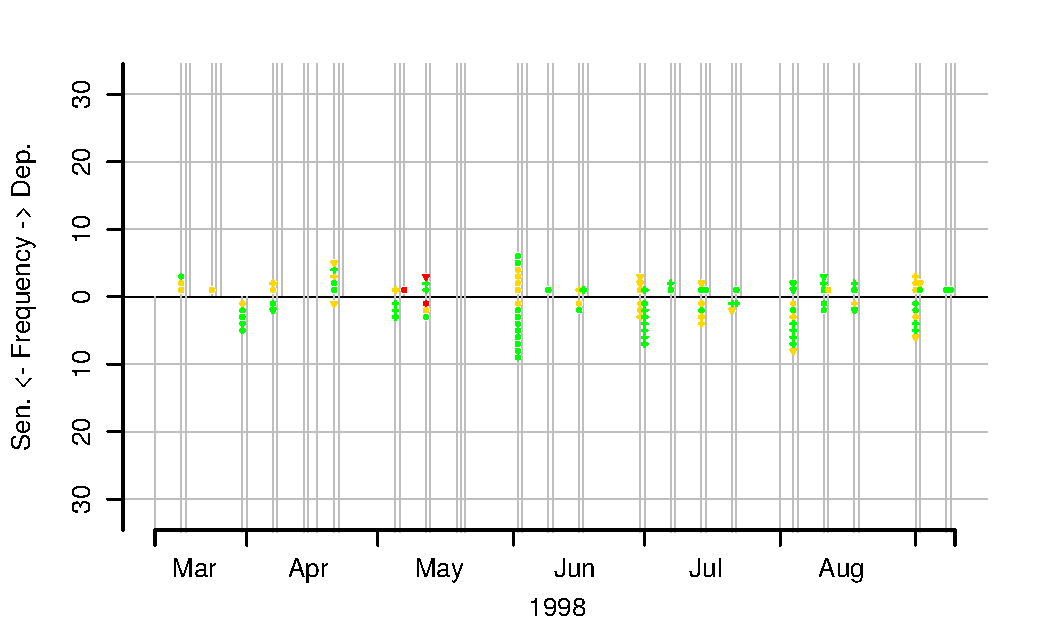
\includegraphics[width=\columnwidth]{../../graphs/urgencias1998-1.pdf} \\

    \begin{tikzpicture}[scale=.1]
      \fill[red]          (0,-1   ) circle (.75);
      \node[right] at     (1.25,-1   ) {\scriptsize{Act now}};  
      \fill[yellow]       (20  ,-1  ) circle (.75);
      \node[right] at     (21.25,-1) {\scriptsize{2-week notice}};  
      \fill[green]        (50  ,-1   ) circle (.75);
      \node[right] at     (51.25,-1 ) {\scriptsize{4-week notice}};  
      \draw[red,thick]    (0  ,-4   )  -- (0,-6);
      \draw[red,thick]    (-1 ,-5   ) -- (1,-5);
      \draw[yellow,thick] (2  ,-4   )  -- (2,-6);
      \draw[yellow,thick] (1  ,-5   ) -- (3,-5);
      \draw[green,thick]  (4  ,-4   )  -- (4,-6);
      \draw[green,thick]  (3  ,-5   ) -- (5,-5);
      \node[right] at     (4.5,-5 ) {\scriptsize{Deadline change}};  
      \fill[red]          (39  ,-4   )  -- (41,-4) -- (40,-6);
      \fill[yellow]       (41  ,-4   )  -- (43,-4) -- (42,-6);
      \fill[green]        (43  ,-4   )  -- (45,-4) -- (44,-6);
      \node[right] at     (44.5,-5  ) {\scriptsize{Withdraw}};  
    \end{tikzpicture}
\end{center}
}
%%%%%%%%%%%%%%%%%%%%%%%%%%%%%%%%%%%%%%%%%%%%%%%%%%%%%%%%%%%%%%%%%%%%%%%%%%%%%%%%%%%%%%%%%%%%%%%%
\frame {                      % SLIDE

    \frametitle{Daily messages 1998--99}

\begin{center}
    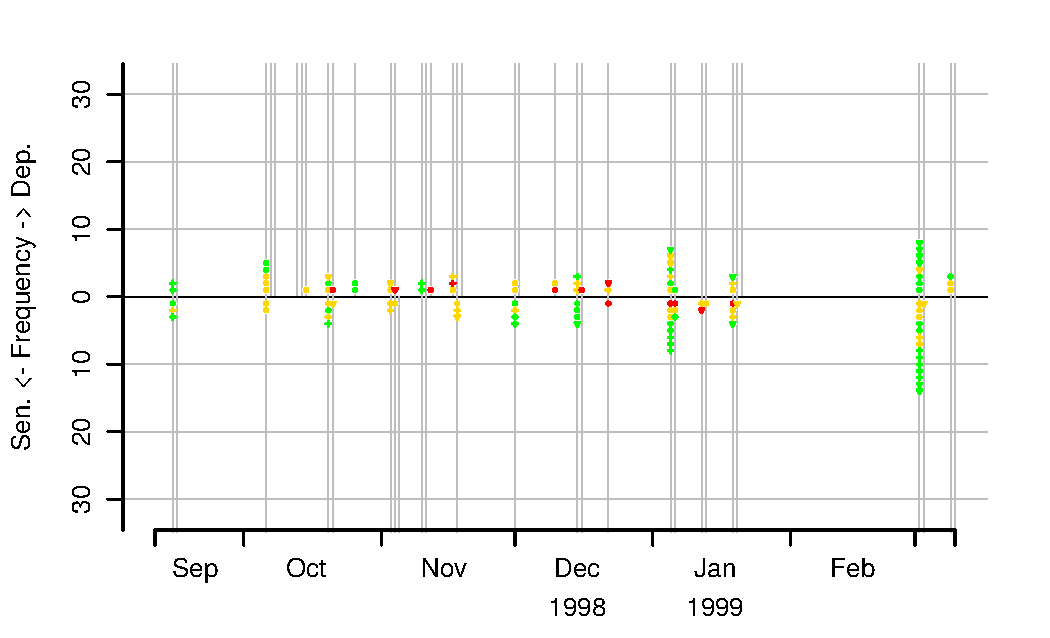
\includegraphics[width=\columnwidth]{../../graphs/urgencias1998-2.pdf} \\

    \begin{tikzpicture}[scale=.1]
      \fill[red]          (0,-1   ) circle (.75);
      \node[right] at     (1.25,-1   ) {\scriptsize{Act now}};  
      \fill[yellow]       (20  ,-1  ) circle (.75);
      \node[right] at     (21.25,-1) {\scriptsize{2-week notice}};  
      \fill[green]        (50  ,-1   ) circle (.75);
      \node[right] at     (51.25,-1 ) {\scriptsize{4-week notice}};  
      \draw[red,thick]    (0  ,-4   )  -- (0,-6);
      \draw[red,thick]    (-1 ,-5   ) -- (1,-5);
      \draw[yellow,thick] (2  ,-4   )  -- (2,-6);
      \draw[yellow,thick] (1  ,-5   ) -- (3,-5);
      \draw[green,thick]  (4  ,-4   )  -- (4,-6);
      \draw[green,thick]  (3  ,-5   ) -- (5,-5);
      \node[right] at     (4.5,-5 ) {\scriptsize{Deadline change}};  
      \fill[red]          (39  ,-4   )  -- (41,-4) -- (40,-6);
      \fill[yellow]       (41  ,-4   )  -- (43,-4) -- (42,-6);
      \fill[green]        (43  ,-4   )  -- (45,-4) -- (44,-6);
      \node[right] at     (44.5,-5  ) {\scriptsize{Withdraw}};  
    \end{tikzpicture}
\end{center}
}
%%%%%%%%%%%%%%%%%%%%%%%%%%%%%%%%%%%%%%%%%%%%%%%%%%%%%%%%%%%%%%%%%%%%%%%%%%%%%%%%%%%%%%%%%%%%%%%%
\frame {                      % SLIDE

    \frametitle{Daily messages 1999--2000}

\begin{center}
    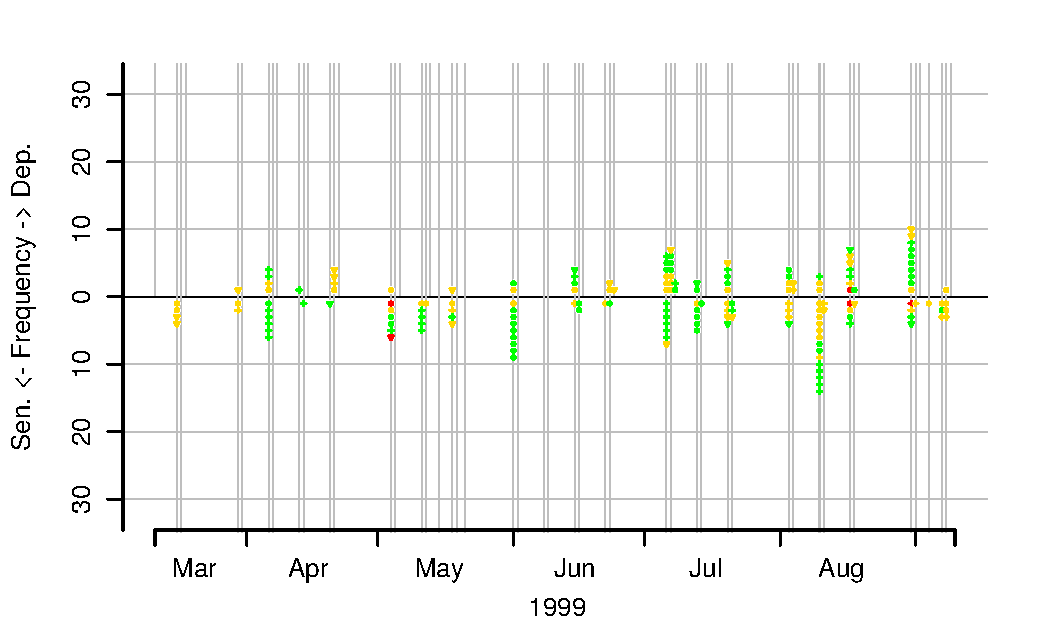
\includegraphics[width=\columnwidth]{../../graphs/urgencias1999-1.pdf} \\

    \begin{tikzpicture}[scale=.1]
      \fill[red]          (0,-1   ) circle (.75);
      \node[right] at     (1.25,-1   ) {\scriptsize{Act now}};  
      \fill[yellow]       (20  ,-1  ) circle (.75);
      \node[right] at     (21.25,-1) {\scriptsize{2-week notice}};  
      \fill[green]        (50  ,-1   ) circle (.75);
      \node[right] at     (51.25,-1 ) {\scriptsize{4-week notice}};  
      \draw[red,thick]    (0  ,-4   )  -- (0,-6);
      \draw[red,thick]    (-1 ,-5   ) -- (1,-5);
      \draw[yellow,thick] (2  ,-4   )  -- (2,-6);
      \draw[yellow,thick] (1  ,-5   ) -- (3,-5);
      \draw[green,thick]  (4  ,-4   )  -- (4,-6);
      \draw[green,thick]  (3  ,-5   ) -- (5,-5);
      \node[right] at     (4.5,-5 ) {\scriptsize{Deadline change}};  
      \fill[red]          (39  ,-4   )  -- (41,-4) -- (40,-6);
      \fill[yellow]       (41  ,-4   )  -- (43,-4) -- (42,-6);
      \fill[green]        (43  ,-4   )  -- (45,-4) -- (44,-6);
      \node[right] at     (44.5,-5  ) {\scriptsize{Withdraw}};  
    \end{tikzpicture}
\end{center}
}
%%%%%%%%%%%%%%%%%%%%%%%%%%%%%%%%%%%%%%%%%%%%%%%%%%%%%%%%%%%%%%%%%%%%%%%%%%%%%%%%%%%%%%%%%%%%%%%%
\frame {                      % SLIDE

    \frametitle{Daily messages 1999--2000}

\begin{center}
    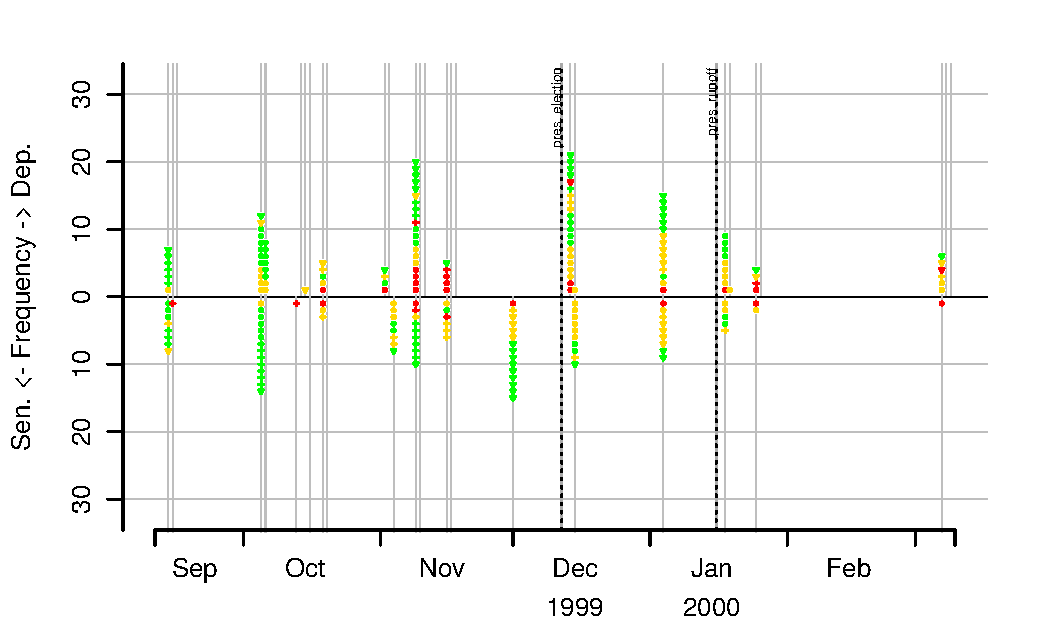
\includegraphics[width=\columnwidth]{../../graphs/urgencias1999-2.pdf} \\

    \begin{tikzpicture}[scale=.1]
      \fill[red]          (0,-1   ) circle (.75);
      \node[right] at     (1.25,-1   ) {\scriptsize{Act now}};  
      \fill[yellow]       (20  ,-1  ) circle (.75);
      \node[right] at     (21.25,-1) {\scriptsize{2-week notice}};  
      \fill[green]        (50  ,-1   ) circle (.75);
      \node[right] at     (51.25,-1 ) {\scriptsize{4-week notice}};  
      \draw[red,thick]    (0  ,-4   )  -- (0,-6);
      \draw[red,thick]    (-1 ,-5   ) -- (1,-5);
      \draw[yellow,thick] (2  ,-4   )  -- (2,-6);
      \draw[yellow,thick] (1  ,-5   ) -- (3,-5);
      \draw[green,thick]  (4  ,-4   )  -- (4,-6);
      \draw[green,thick]  (3  ,-5   ) -- (5,-5);
      \node[right] at     (4.5,-5 ) {\scriptsize{Deadline change}};  
      \fill[red]          (39  ,-4   )  -- (41,-4) -- (40,-6);
      \fill[yellow]       (41  ,-4   )  -- (43,-4) -- (42,-6);
      \fill[green]        (43  ,-4   )  -- (45,-4) -- (44,-6);
      \node[right] at     (44.5,-5  ) {\scriptsize{Withdraw}};  
    \end{tikzpicture}
\end{center}
}
%%%%%%%%%%%%%%%%%%%%%%%%%%%%%%%%%%%%%%%%%%%%%%%%%%%%%%%%%%%%%%%%%%%%%%%%%%%%%%%%%%%%%%%%%%%%%%%%
\frame {                      % SLIDE

    \frametitle{Daily messages 2000--01}

\begin{center}
    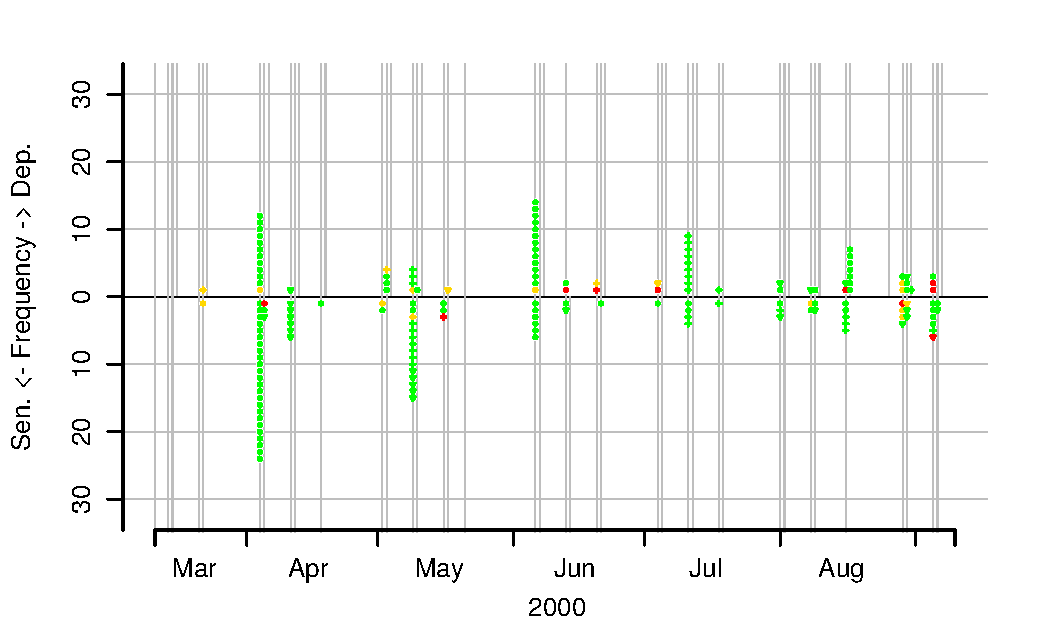
\includegraphics[width=\columnwidth]{../../graphs/urgencias2000-1.pdf} \\

    \begin{tikzpicture}[scale=.1]
      \fill[red]          (0,-1   ) circle (.75);
      \node[right] at     (1.25,-1   ) {\scriptsize{Act now}};  
      \fill[yellow]       (20  ,-1  ) circle (.75);
      \node[right] at     (21.25,-1) {\scriptsize{2-week notice}};  
      \fill[green]        (50  ,-1   ) circle (.75);
      \node[right] at     (51.25,-1 ) {\scriptsize{4-week notice}};  
      \draw[red,thick]    (0  ,-4   )  -- (0,-6);
      \draw[red,thick]    (-1 ,-5   ) -- (1,-5);
      \draw[yellow,thick] (2  ,-4   )  -- (2,-6);
      \draw[yellow,thick] (1  ,-5   ) -- (3,-5);
      \draw[green,thick]  (4  ,-4   )  -- (4,-6);
      \draw[green,thick]  (3  ,-5   ) -- (5,-5);
      \node[right] at     (4.5,-5 ) {\scriptsize{Deadline change}};  
      \fill[red]          (39  ,-4   )  -- (41,-4) -- (40,-6);
      \fill[yellow]       (41  ,-4   )  -- (43,-4) -- (42,-6);
      \fill[green]        (43  ,-4   )  -- (45,-4) -- (44,-6);
      \node[right] at     (44.5,-5  ) {\scriptsize{Withdraw}};  
    \end{tikzpicture}
\end{center}
}
%%%%%%%%%%%%%%%%%%%%%%%%%%%%%%%%%%%%%%%%%%%%%%%%%%%%%%%%%%%%%%%%%%%%%%%%%%%%%%%%%%%%%%%%%%%%%%%%
\frame {                      % SLIDE

    \frametitle{Daily messages 2000--01}

\begin{center}
    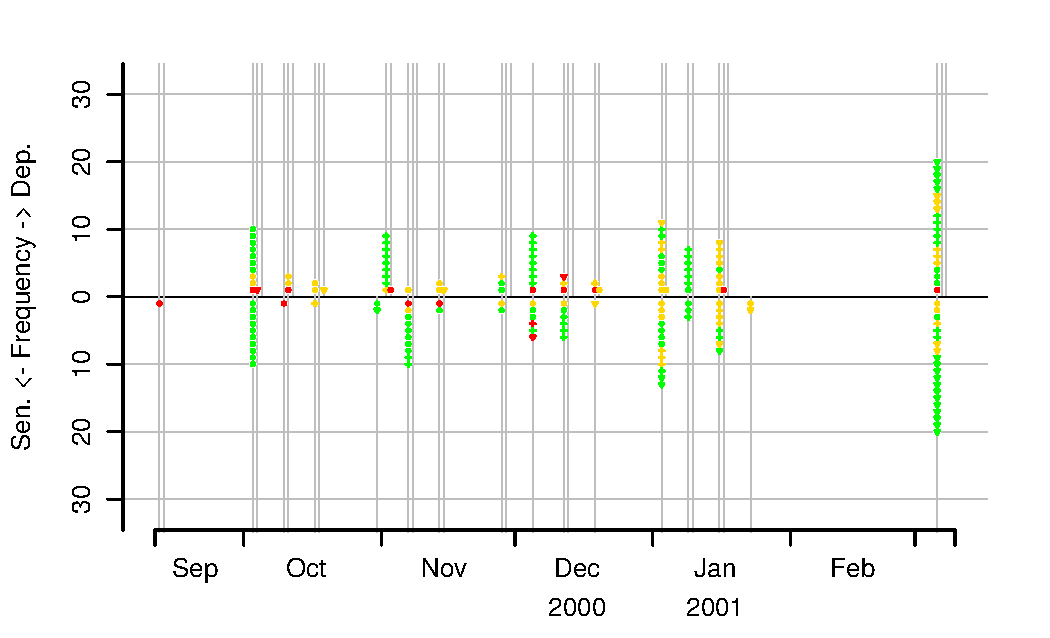
\includegraphics[width=\columnwidth]{../../graphs/urgencias2000-2.pdf} \\

    \begin{tikzpicture}[scale=.1]
      \fill[red]          (0,-1   ) circle (.75);
      \node[right] at     (1.25,-1   ) {\scriptsize{Act now}};  
      \fill[yellow]       (20  ,-1  ) circle (.75);
      \node[right] at     (21.25,-1) {\scriptsize{2-week notice}};  
      \fill[green]        (50  ,-1   ) circle (.75);
      \node[right] at     (51.25,-1 ) {\scriptsize{4-week notice}};  
      \draw[red,thick]    (0  ,-4   )  -- (0,-6);
      \draw[red,thick]    (-1 ,-5   ) -- (1,-5);
      \draw[yellow,thick] (2  ,-4   )  -- (2,-6);
      \draw[yellow,thick] (1  ,-5   ) -- (3,-5);
      \draw[green,thick]  (4  ,-4   )  -- (4,-6);
      \draw[green,thick]  (3  ,-5   ) -- (5,-5);
      \node[right] at     (4.5,-5 ) {\scriptsize{Deadline change}};  
      \fill[red]          (39  ,-4   )  -- (41,-4) -- (40,-6);
      \fill[yellow]       (41  ,-4   )  -- (43,-4) -- (42,-6);
      \fill[green]        (43  ,-4   )  -- (45,-4) -- (44,-6);
      \node[right] at     (44.5,-5  ) {\scriptsize{Withdraw}};  
    \end{tikzpicture}
\end{center}
}
%%%%%%%%%%%%%%%%%%%%%%%%%%%%%%%%%%%%%%%%%%%%%%%%%%%%%%%%%%%%%%%%%%%%%%%%%%%%%%%%%%%%%%%%%%%%%%%%
\frame {                      % SLIDE

    \frametitle{Daily messages 2001--02}

\begin{center}
    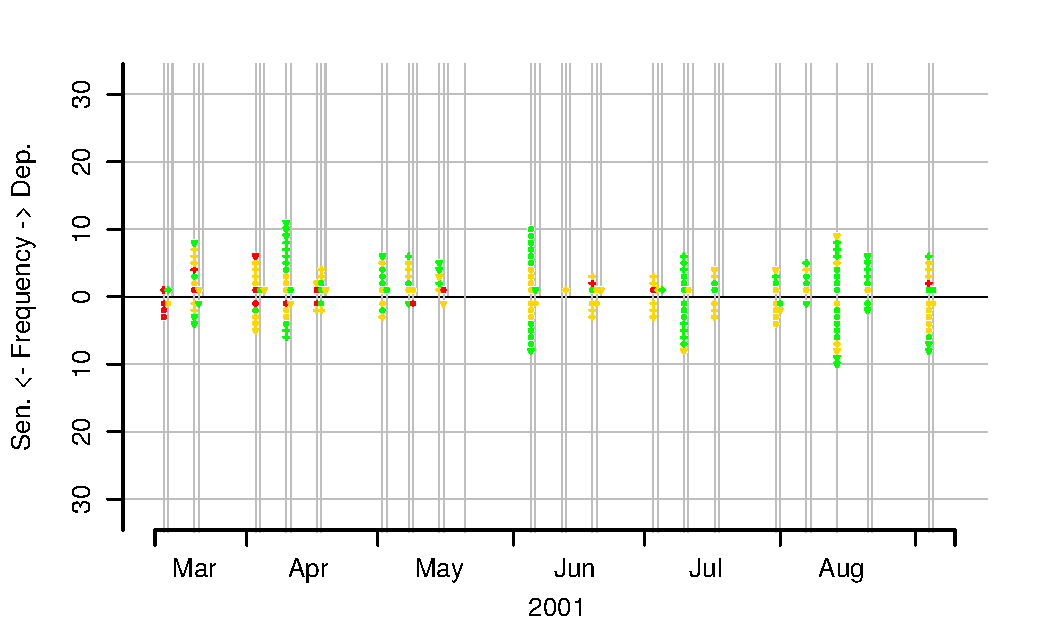
\includegraphics[width=\columnwidth]{../../graphs/urgencias2001-1.pdf} \\

    \begin{tikzpicture}[scale=.1]
      \fill[red]          (0,-1   ) circle (.75);
      \node[right] at     (1.25,-1   ) {\scriptsize{Act now}};  
      \fill[yellow]       (20  ,-1  ) circle (.75);
      \node[right] at     (21.25,-1) {\scriptsize{2-week notice}};  
      \fill[green]        (50  ,-1   ) circle (.75);
      \node[right] at     (51.25,-1 ) {\scriptsize{4-week notice}};  
      \draw[red,thick]    (0  ,-4   )  -- (0,-6);
      \draw[red,thick]    (-1 ,-5   ) -- (1,-5);
      \draw[yellow,thick] (2  ,-4   )  -- (2,-6);
      \draw[yellow,thick] (1  ,-5   ) -- (3,-5);
      \draw[green,thick]  (4  ,-4   )  -- (4,-6);
      \draw[green,thick]  (3  ,-5   ) -- (5,-5);
      \node[right] at     (4.5,-5 ) {\scriptsize{Deadline change}};  
      \fill[red]          (39  ,-4   )  -- (41,-4) -- (40,-6);
      \fill[yellow]       (41  ,-4   )  -- (43,-4) -- (42,-6);
      \fill[green]        (43  ,-4   )  -- (45,-4) -- (44,-6);
      \node[right] at     (44.5,-5  ) {\scriptsize{Withdraw}};  
    \end{tikzpicture}
\end{center}
}
%%%%%%%%%%%%%%%%%%%%%%%%%%%%%%%%%%%%%%%%%%%%%%%%%%%%%%%%%%%%%%%%%%%%%%%%%%%%%%%%%%%%%%%%%%%%%%%%
\frame {                      % SLIDE

    \frametitle{Daily messages 2001--02}

\begin{center}
    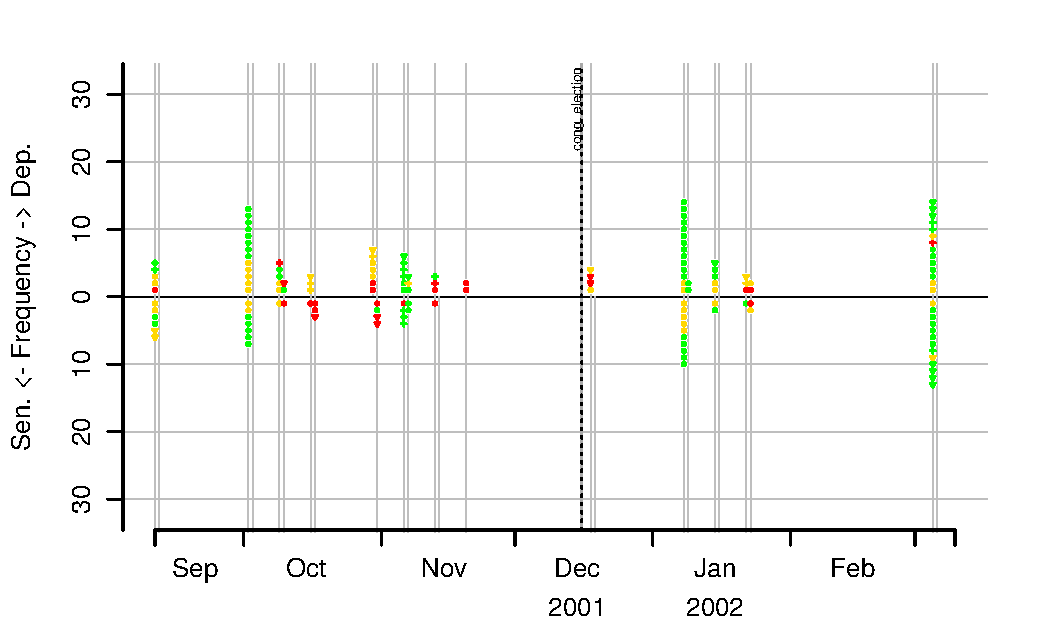
\includegraphics[width=\columnwidth]{../../graphs/urgencias2001-2.pdf} \\

    \begin{tikzpicture}[scale=.1]
      \fill[red]          (0,-1   ) circle (.75);
      \node[right] at     (1.25,-1   ) {\scriptsize{Act now}};  
      \fill[yellow]       (20  ,-1  ) circle (.75);
      \node[right] at     (21.25,-1) {\scriptsize{2-week notice}};  
      \fill[green]        (50  ,-1   ) circle (.75);
      \node[right] at     (51.25,-1 ) {\scriptsize{4-week notice}};  
      \draw[red,thick]    (0  ,-4   )  -- (0,-6);
      \draw[red,thick]    (-1 ,-5   ) -- (1,-5);
      \draw[yellow,thick] (2  ,-4   )  -- (2,-6);
      \draw[yellow,thick] (1  ,-5   ) -- (3,-5);
      \draw[green,thick]  (4  ,-4   )  -- (4,-6);
      \draw[green,thick]  (3  ,-5   ) -- (5,-5);
      \node[right] at     (4.5,-5 ) {\scriptsize{Deadline change}};  
      \fill[red]          (39  ,-4   )  -- (41,-4) -- (40,-6);
      \fill[yellow]       (41  ,-4   )  -- (43,-4) -- (42,-6);
      \fill[green]        (43  ,-4   )  -- (45,-4) -- (44,-6);
      \node[right] at     (44.5,-5  ) {\scriptsize{Withdraw}};  
    \end{tikzpicture}
\end{center}
}
%%%%%%%%%%%%%%%%%%%%%%%%%%%%%%%%%%%%%%%%%%%%%%%%%%%%%%%%%%%%%%%%%%%%%%%%%%%%%%%%%%%%%%%%%%%%%%%%
\frame {                      % SLIDE

    \frametitle{Daily messages 2002--03}

\begin{center}
    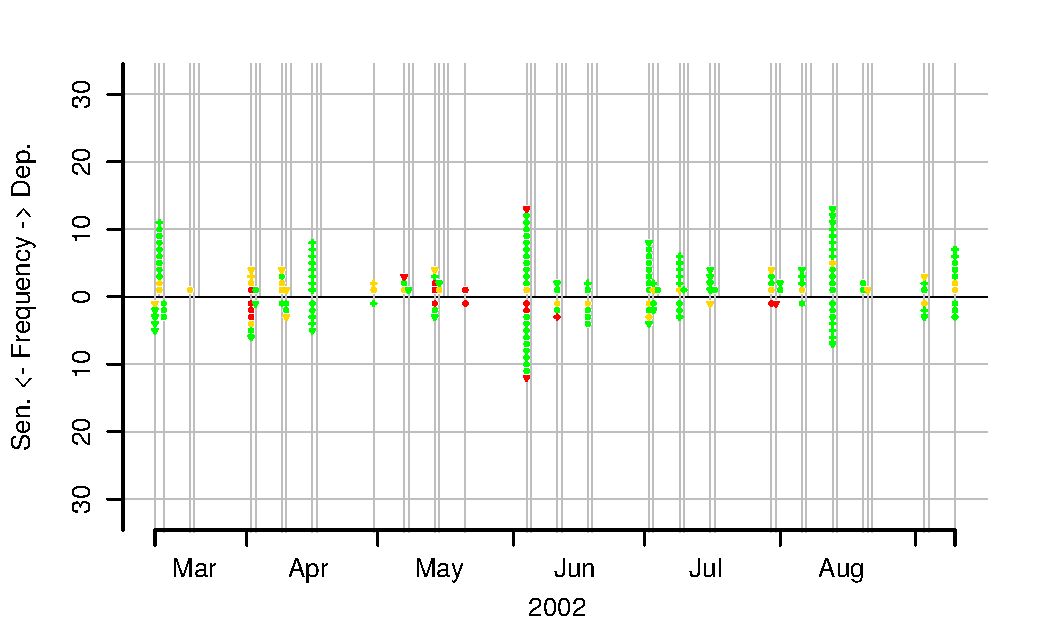
\includegraphics[width=\columnwidth]{../../graphs/urgencias2002-1.pdf} \\

    \begin{tikzpicture}[scale=.1]
      \fill[red]          (0,-1   ) circle (.75);
      \node[right] at     (1.25,-1   ) {\scriptsize{Act now}};  
      \fill[yellow]       (20  ,-1  ) circle (.75);
      \node[right] at     (21.25,-1) {\scriptsize{2-week notice}};  
      \fill[green]        (50  ,-1   ) circle (.75);
      \node[right] at     (51.25,-1 ) {\scriptsize{4-week notice}};  
      \draw[red,thick]    (0  ,-4   )  -- (0,-6);
      \draw[red,thick]    (-1 ,-5   ) -- (1,-5);
      \draw[yellow,thick] (2  ,-4   )  -- (2,-6);
      \draw[yellow,thick] (1  ,-5   ) -- (3,-5);
      \draw[green,thick]  (4  ,-4   )  -- (4,-6);
      \draw[green,thick]  (3  ,-5   ) -- (5,-5);
      \node[right] at     (4.5,-5 ) {\scriptsize{Deadline change}};  
      \fill[red]          (39  ,-4   )  -- (41,-4) -- (40,-6);
      \fill[yellow]       (41  ,-4   )  -- (43,-4) -- (42,-6);
      \fill[green]        (43  ,-4   )  -- (45,-4) -- (44,-6);
      \node[right] at     (44.5,-5  ) {\scriptsize{Withdraw}};  
    \end{tikzpicture}
\end{center}
}
%%%%%%%%%%%%%%%%%%%%%%%%%%%%%%%%%%%%%%%%%%%%%%%%%%%%%%%%%%%%%%%%%%%%%%%%%%%%%%%%%%%%%%%%%%%%%%%%
\frame {                      % SLIDE

    \frametitle{Daily messages 2002--03}

\begin{center}
    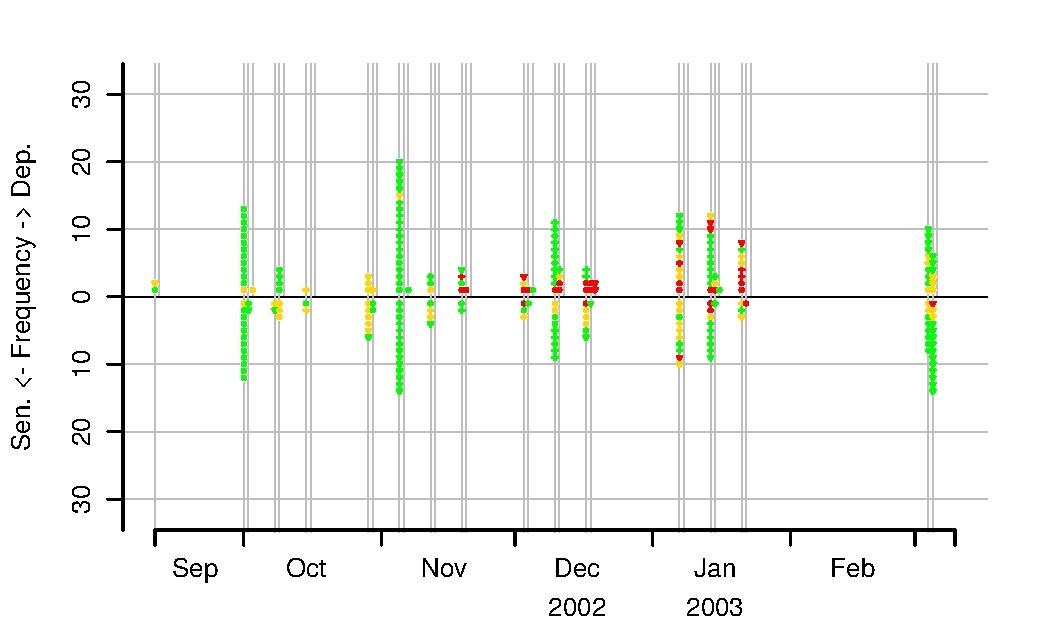
\includegraphics[width=\columnwidth]{../../graphs/urgencias2002-2.pdf} \\

    \begin{tikzpicture}[scale=.1]
      \fill[red]          (0,-1   ) circle (.75);
      \node[right] at     (1.25,-1   ) {\scriptsize{Act now}};  
      \fill[yellow]       (20  ,-1  ) circle (.75);
      \node[right] at     (21.25,-1) {\scriptsize{2-week notice}};  
      \fill[green]        (50  ,-1   ) circle (.75);
      \node[right] at     (51.25,-1 ) {\scriptsize{4-week notice}};  
      \draw[red,thick]    (0  ,-4   )  -- (0,-6);
      \draw[red,thick]    (-1 ,-5   ) -- (1,-5);
      \draw[yellow,thick] (2  ,-4   )  -- (2,-6);
      \draw[yellow,thick] (1  ,-5   ) -- (3,-5);
      \draw[green,thick]  (4  ,-4   )  -- (4,-6);
      \draw[green,thick]  (3  ,-5   ) -- (5,-5);
      \node[right] at     (4.5,-5 ) {\scriptsize{Deadline change}};  
      \fill[red]          (39  ,-4   )  -- (41,-4) -- (40,-6);
      \fill[yellow]       (41  ,-4   )  -- (43,-4) -- (42,-6);
      \fill[green]        (43  ,-4   )  -- (45,-4) -- (44,-6);
      \node[right] at     (44.5,-5  ) {\scriptsize{Withdraw}};  
    \end{tikzpicture}
\end{center}
}
%%%%%%%%%%%%%%%%%%%%%%%%%%%%%%%%%%%%%%%%%%%%%%%%%%%%%%%%%%%%%%%%%%%%%%%%%%%%%%%%%%%%%%%%%%%%%%%%
\frame {                      % SLIDE

    \frametitle{Daily messages 2003--04}

\begin{center}
    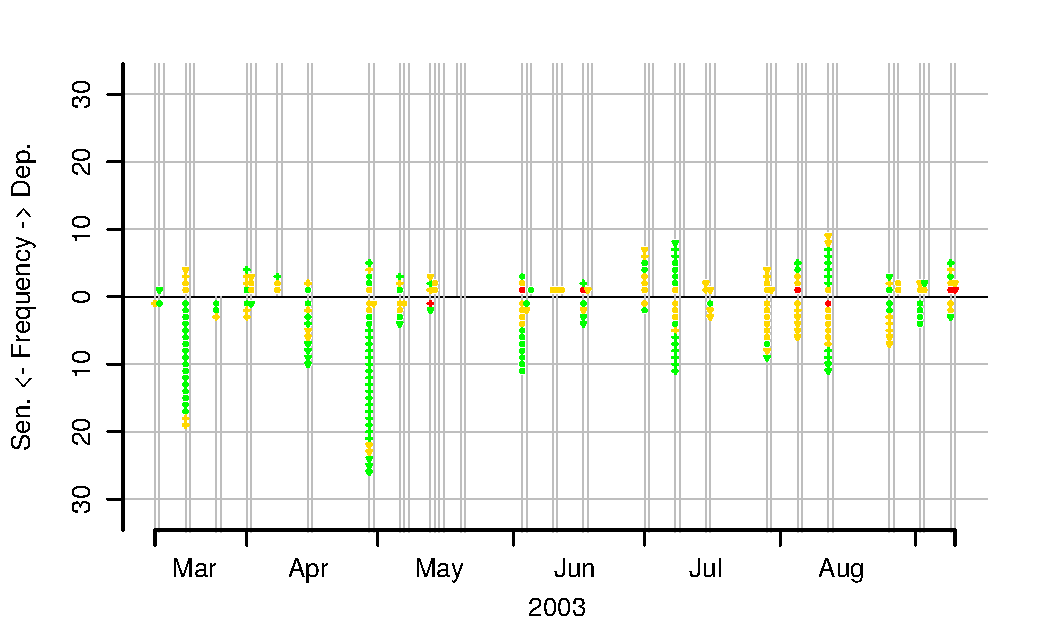
\includegraphics[width=\columnwidth]{../../graphs/urgencias2003-1.pdf} \\

    \begin{tikzpicture}[scale=.1]
      \fill[red]          (0,-1   ) circle (.75);
      \node[right] at     (1.25,-1   ) {\scriptsize{Act now}};  
      \fill[yellow]       (20  ,-1  ) circle (.75);
      \node[right] at     (21.25,-1) {\scriptsize{2-week notice}};  
      \fill[green]        (50  ,-1   ) circle (.75);
      \node[right] at     (51.25,-1 ) {\scriptsize{4-week notice}};  
      \draw[red,thick]    (0  ,-4   )  -- (0,-6);
      \draw[red,thick]    (-1 ,-5   ) -- (1,-5);
      \draw[yellow,thick] (2  ,-4   )  -- (2,-6);
      \draw[yellow,thick] (1  ,-5   ) -- (3,-5);
      \draw[green,thick]  (4  ,-4   )  -- (4,-6);
      \draw[green,thick]  (3  ,-5   ) -- (5,-5);
      \node[right] at     (4.5,-5 ) {\scriptsize{Deadline change}};  
      \fill[red]          (39  ,-4   )  -- (41,-4) -- (40,-6);
      \fill[yellow]       (41  ,-4   )  -- (43,-4) -- (42,-6);
      \fill[green]        (43  ,-4   )  -- (45,-4) -- (44,-6);
      \node[right] at     (44.5,-5  ) {\scriptsize{Withdraw}};  
    \end{tikzpicture}
\end{center}
}
%%%%%%%%%%%%%%%%%%%%%%%%%%%%%%%%%%%%%%%%%%%%%%%%%%%%%%%%%%%%%%%%%%%%%%%%%%%%%%%%%%%%%%%%%%%%%%%%
\frame {                      % SLIDE

    \frametitle{Daily messages 2003--04}

\begin{center}
    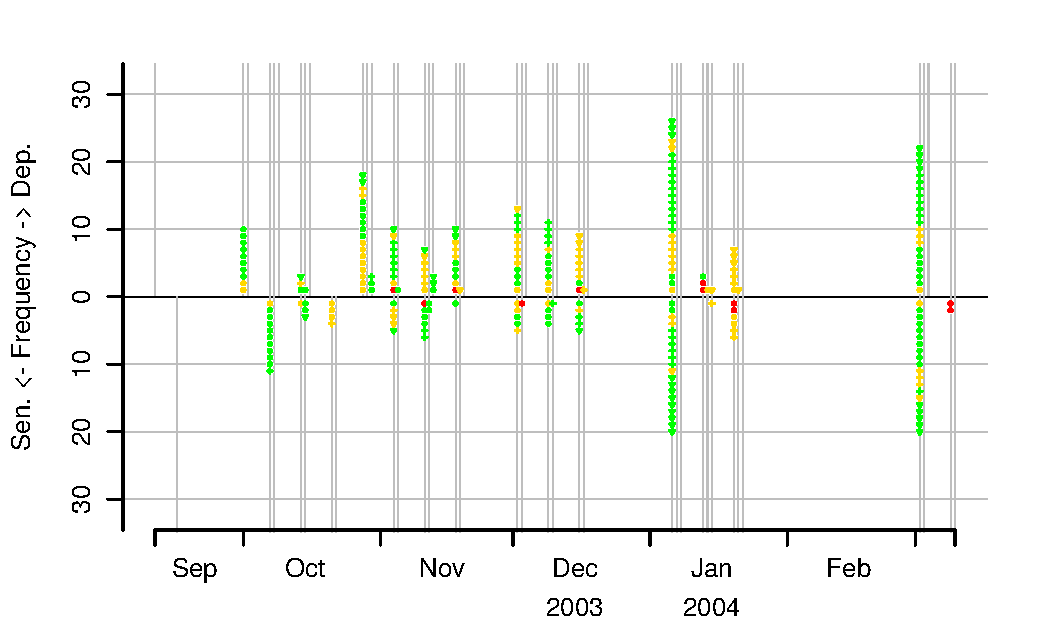
\includegraphics[width=\columnwidth]{../../graphs/urgencias2003-2.pdf} \\

    \begin{tikzpicture}[scale=.1]
      \fill[red]          (0,-1   ) circle (.75);
      \node[right] at     (1.25,-1   ) {\scriptsize{Act now}};  
      \fill[yellow]       (20  ,-1  ) circle (.75);
      \node[right] at     (21.25,-1) {\scriptsize{2-week notice}};  
      \fill[green]        (50  ,-1   ) circle (.75);
      \node[right] at     (51.25,-1 ) {\scriptsize{4-week notice}};  
      \draw[red,thick]    (0  ,-4   )  -- (0,-6);
      \draw[red,thick]    (-1 ,-5   ) -- (1,-5);
      \draw[yellow,thick] (2  ,-4   )  -- (2,-6);
      \draw[yellow,thick] (1  ,-5   ) -- (3,-5);
      \draw[green,thick]  (4  ,-4   )  -- (4,-6);
      \draw[green,thick]  (3  ,-5   ) -- (5,-5);
      \node[right] at     (4.5,-5 ) {\scriptsize{Deadline change}};  
      \fill[red]          (39  ,-4   )  -- (41,-4) -- (40,-6);
      \fill[yellow]       (41  ,-4   )  -- (43,-4) -- (42,-6);
      \fill[green]        (43  ,-4   )  -- (45,-4) -- (44,-6);
      \node[right] at     (44.5,-5  ) {\scriptsize{Withdraw}};  
    \end{tikzpicture}
\end{center}
}
%%%%%%%%%%%%%%%%%%%%%%%%%%%%%%%%%%%%%%%%%%%%%%%%%%%%%%%%%%%%%%%%%%%%%%%%%%%%%%%%%%%%%%%%%%%%%%%%
\frame {                      % SLIDE

    \frametitle{Daily messages 2004--05}

\begin{center}
    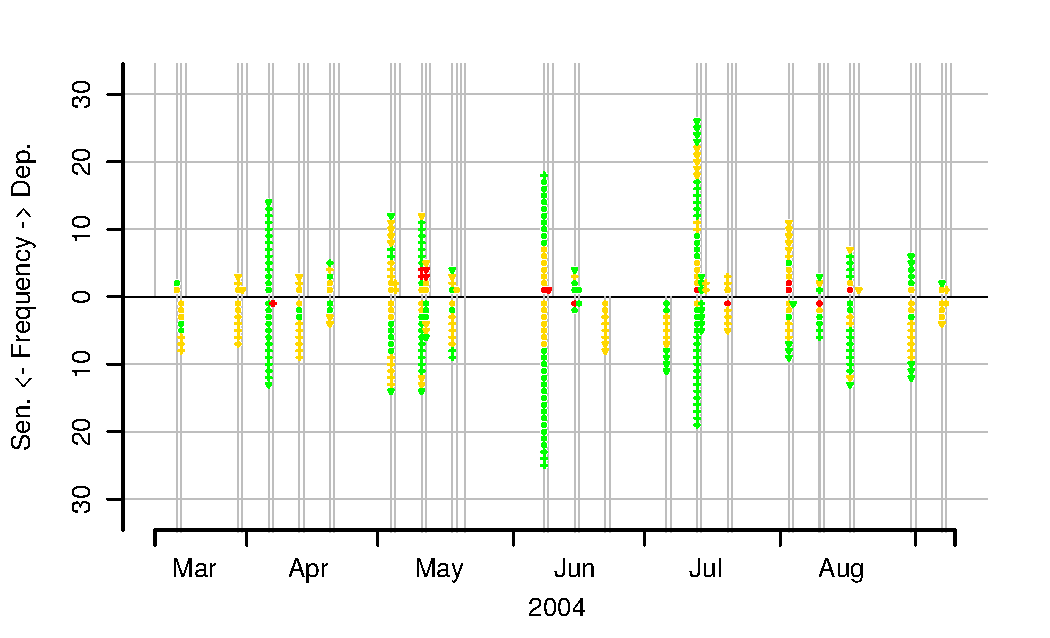
\includegraphics[width=\columnwidth]{../../graphs/urgencias2004-1.pdf} \\

    \begin{tikzpicture}[scale=.1]
      \fill[red]          (0,-1   ) circle (.75);
      \node[right] at     (1.25,-1   ) {\scriptsize{Act now}};  
      \fill[yellow]       (20  ,-1  ) circle (.75);
      \node[right] at     (21.25,-1) {\scriptsize{2-week notice}};  
      \fill[green]        (50  ,-1   ) circle (.75);
      \node[right] at     (51.25,-1 ) {\scriptsize{4-week notice}};  
      \draw[red,thick]    (0  ,-4   )  -- (0,-6);
      \draw[red,thick]    (-1 ,-5   ) -- (1,-5);
      \draw[yellow,thick] (2  ,-4   )  -- (2,-6);
      \draw[yellow,thick] (1  ,-5   ) -- (3,-5);
      \draw[green,thick]  (4  ,-4   )  -- (4,-6);
      \draw[green,thick]  (3  ,-5   ) -- (5,-5);
      \node[right] at     (4.5,-5 ) {\scriptsize{Deadline change}};  
      \fill[red]          (39  ,-4   )  -- (41,-4) -- (40,-6);
      \fill[yellow]       (41  ,-4   )  -- (43,-4) -- (42,-6);
      \fill[green]        (43  ,-4   )  -- (45,-4) -- (44,-6);
      \node[right] at     (44.5,-5  ) {\scriptsize{Withdraw}};  
    \end{tikzpicture}
\end{center}
}
%%%%%%%%%%%%%%%%%%%%%%%%%%%%%%%%%%%%%%%%%%%%%%%%%%%%%%%%%%%%%%%%%%%%%%%%%%%%%%%%%%%%%%%%%%%%%%%%
\frame {                      % SLIDE

    \frametitle{Daily messages 2004--05}

\begin{center}
    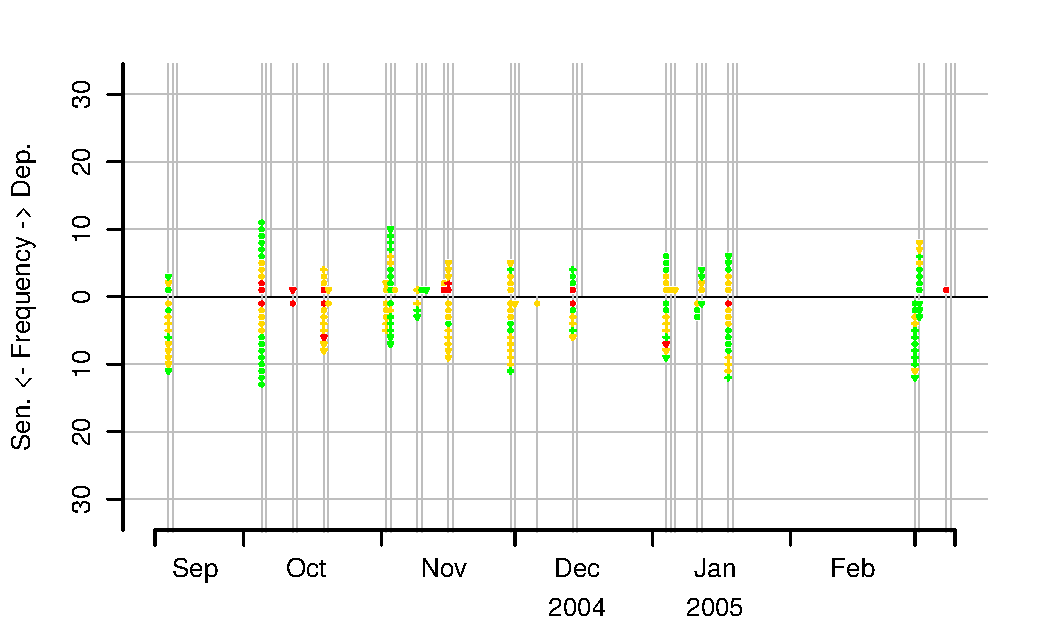
\includegraphics[width=\columnwidth]{../../graphs/urgencias2004-2.pdf} \\

    \begin{tikzpicture}[scale=.1]
      \fill[red]          (0,-1   ) circle (.75);
      \node[right] at     (1.25,-1   ) {\scriptsize{Act now}};  
      \fill[yellow]       (20  ,-1  ) circle (.75);
      \node[right] at     (21.25,-1) {\scriptsize{2-week notice}};  
      \fill[green]        (50  ,-1   ) circle (.75);
      \node[right] at     (51.25,-1 ) {\scriptsize{4-week notice}};  
      \draw[red,thick]    (0  ,-4   )  -- (0,-6);
      \draw[red,thick]    (-1 ,-5   ) -- (1,-5);
      \draw[yellow,thick] (2  ,-4   )  -- (2,-6);
      \draw[yellow,thick] (1  ,-5   ) -- (3,-5);
      \draw[green,thick]  (4  ,-4   )  -- (4,-6);
      \draw[green,thick]  (3  ,-5   ) -- (5,-5);
      \node[right] at     (4.5,-5 ) {\scriptsize{Deadline change}};  
      \fill[red]          (39  ,-4   )  -- (41,-4) -- (40,-6);
      \fill[yellow]       (41  ,-4   )  -- (43,-4) -- (42,-6);
      \fill[green]        (43  ,-4   )  -- (45,-4) -- (44,-6);
      \node[right] at     (44.5,-5  ) {\scriptsize{Withdraw}};  
    \end{tikzpicture}
\end{center}
}
%%%%%%%%%%%%%%%%%%%%%%%%%%%%%%%%%%%%%%%%%%%%%%%%%%%%%%%%%%%%%%%%%%%%%%%%%%%%%%%%%%%%%%%%%%%%%%%%
\frame {                      % SLIDE

    \frametitle{Daily messages 2005--06}

\begin{center}
    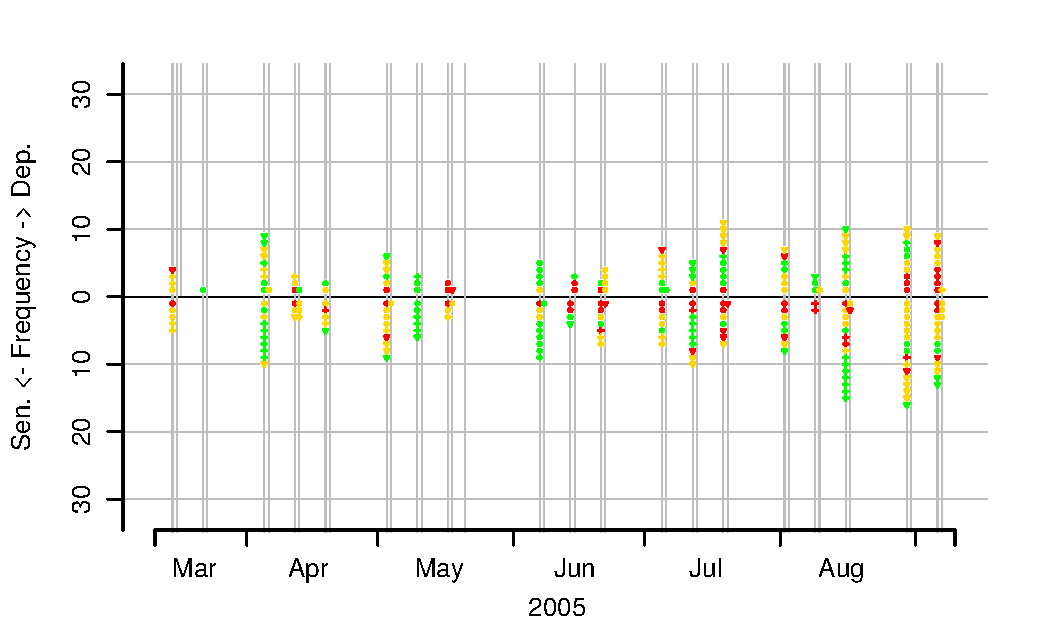
\includegraphics[width=\columnwidth]{../../graphs/urgencias2005-1.pdf} \\

    \begin{tikzpicture}[scale=.1]
      \fill[red]          (0,-1   ) circle (.75);
      \node[right] at     (1.25,-1   ) {\scriptsize{Act now}};  
      \fill[yellow]       (20  ,-1  ) circle (.75);
      \node[right] at     (21.25,-1) {\scriptsize{2-week notice}};  
      \fill[green]        (50  ,-1   ) circle (.75);
      \node[right] at     (51.25,-1 ) {\scriptsize{4-week notice}};  
      \draw[red,thick]    (0  ,-4   )  -- (0,-6);
      \draw[red,thick]    (-1 ,-5   ) -- (1,-5);
      \draw[yellow,thick] (2  ,-4   )  -- (2,-6);
      \draw[yellow,thick] (1  ,-5   ) -- (3,-5);
      \draw[green,thick]  (4  ,-4   )  -- (4,-6);
      \draw[green,thick]  (3  ,-5   ) -- (5,-5);
      \node[right] at     (4.5,-5 ) {\scriptsize{Deadline change}};  
      \fill[red]          (39  ,-4   )  -- (41,-4) -- (40,-6);
      \fill[yellow]       (41  ,-4   )  -- (43,-4) -- (42,-6);
      \fill[green]        (43  ,-4   )  -- (45,-4) -- (44,-6);
      \node[right] at     (44.5,-5  ) {\scriptsize{Withdraw}};  
    \end{tikzpicture}
\end{center}
}
%%%%%%%%%%%%%%%%%%%%%%%%%%%%%%%%%%%%%%%%%%%%%%%%%%%%%%%%%%%%%%%%%%%%%%%%%%%%%%%%%%%%%%%%%%%%%%%%
\frame {                      % SLIDE

    \frametitle{Daily messages 2005--06}

\begin{center}
    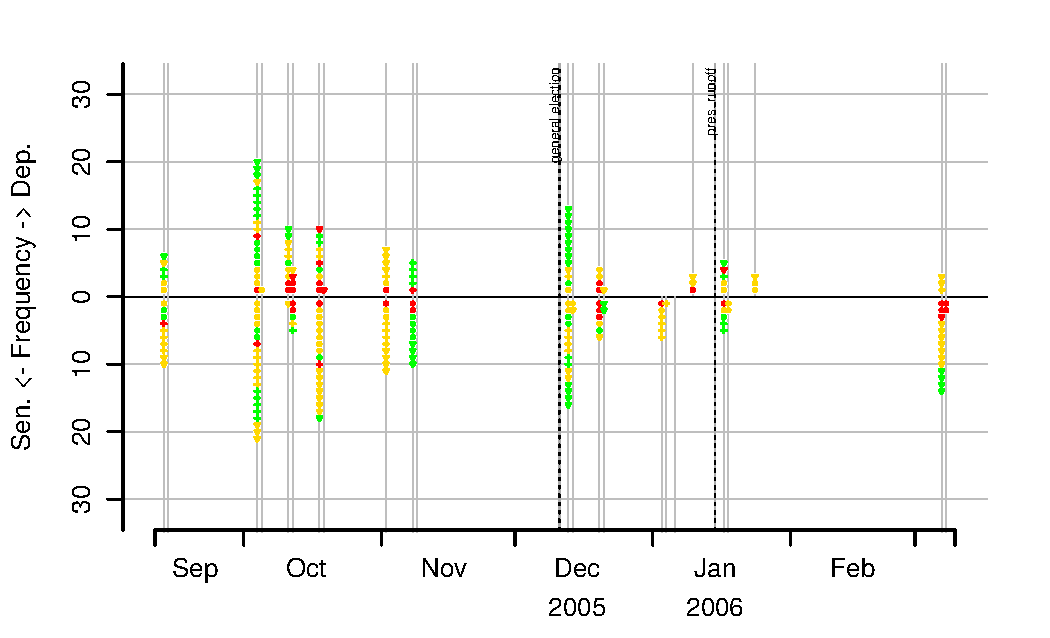
\includegraphics[width=\columnwidth]{../../graphs/urgencias2005-2.pdf} \\

    \begin{tikzpicture}[scale=.1]
      \fill[red]          (0,-1   ) circle (.75);
      \node[right] at     (1.25,-1   ) {\scriptsize{Act now}};  
      \fill[yellow]       (20  ,-1  ) circle (.75);
      \node[right] at     (21.25,-1) {\scriptsize{2-week notice}};  
      \fill[green]        (50  ,-1   ) circle (.75);
      \node[right] at     (51.25,-1 ) {\scriptsize{4-week notice}};  
      \draw[red,thick]    (0  ,-4   )  -- (0,-6);
      \draw[red,thick]    (-1 ,-5   ) -- (1,-5);
      \draw[yellow,thick] (2  ,-4   )  -- (2,-6);
      \draw[yellow,thick] (1  ,-5   ) -- (3,-5);
      \draw[green,thick]  (4  ,-4   )  -- (4,-6);
      \draw[green,thick]  (3  ,-5   ) -- (5,-5);
      \node[right] at     (4.5,-5 ) {\scriptsize{Deadline change}};  
      \fill[red]          (39  ,-4   )  -- (41,-4) -- (40,-6);
      \fill[yellow]       (41  ,-4   )  -- (43,-4) -- (42,-6);
      \fill[green]        (43  ,-4   )  -- (45,-4) -- (44,-6);
      \node[right] at     (44.5,-5  ) {\scriptsize{Withdraw}};  
    \end{tikzpicture}
\end{center}
}
%%%%%%%%%%%%%%%%%%%%%%%%%%%%%%%%%%%%%%%%%%%%%%%%%%%%%%%%%%%%%%%%%%%%%%%%%%%%%%%%%%%%%%%%%%%%%%%%
\frame {                      % SLIDE

    \frametitle{Daily messages 2006--07}

\begin{center}
    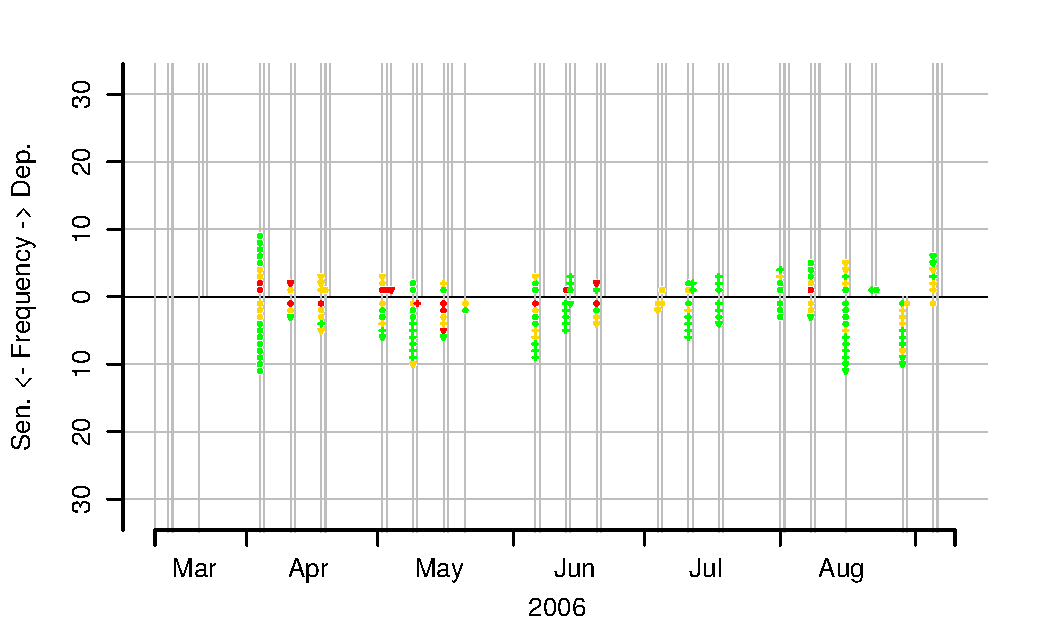
\includegraphics[width=\columnwidth]{../../graphs/urgencias2006-1.pdf} \\

    \begin{tikzpicture}[scale=.1]
      \fill[red]          (0,-1   ) circle (.75);
      \node[right] at     (1.25,-1   ) {\scriptsize{Act now}};  
      \fill[yellow]       (20  ,-1  ) circle (.75);
      \node[right] at     (21.25,-1) {\scriptsize{2-week notice}};  
      \fill[green]        (50  ,-1   ) circle (.75);
      \node[right] at     (51.25,-1 ) {\scriptsize{4-week notice}};  
      \draw[red,thick]    (0  ,-4   )  -- (0,-6);
      \draw[red,thick]    (-1 ,-5   ) -- (1,-5);
      \draw[yellow,thick] (2  ,-4   )  -- (2,-6);
      \draw[yellow,thick] (1  ,-5   ) -- (3,-5);
      \draw[green,thick]  (4  ,-4   )  -- (4,-6);
      \draw[green,thick]  (3  ,-5   ) -- (5,-5);
      \node[right] at     (4.5,-5 ) {\scriptsize{Deadline change}};  
      \fill[red]          (39  ,-4   )  -- (41,-4) -- (40,-6);
      \fill[yellow]       (41  ,-4   )  -- (43,-4) -- (42,-6);
      \fill[green]        (43  ,-4   )  -- (45,-4) -- (44,-6);
      \node[right] at     (44.5,-5  ) {\scriptsize{Withdraw}};  
    \end{tikzpicture}
\end{center}
}
%%%%%%%%%%%%%%%%%%%%%%%%%%%%%%%%%%%%%%%%%%%%%%%%%%%%%%%%%%%%%%%%%%%%%%%%%%%%%%%%%%%%%%%%%%%%%%%%
\frame {                      % SLIDE

    \frametitle{Daily messages 2006--07}

\begin{center}
    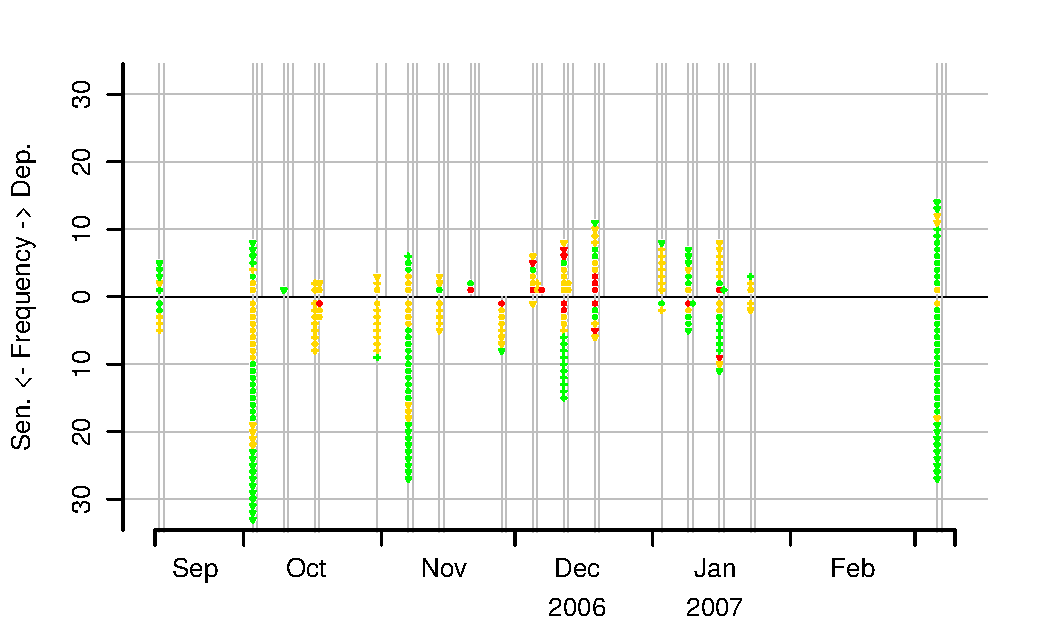
\includegraphics[width=\columnwidth]{../../graphs/urgencias2006-2.pdf} \\

    \begin{tikzpicture}[scale=.1]
      \fill[red]          (0,-1   ) circle (.75);
      \node[right] at     (1.25,-1   ) {\scriptsize{Act now}};  
      \fill[yellow]       (20  ,-1  ) circle (.75);
      \node[right] at     (21.25,-1) {\scriptsize{2-week notice}};  
      \fill[green]        (50  ,-1   ) circle (.75);
      \node[right] at     (51.25,-1 ) {\scriptsize{4-week notice}};  
      \draw[red,thick]    (0  ,-4   )  -- (0,-6);
      \draw[red,thick]    (-1 ,-5   ) -- (1,-5);
      \draw[yellow,thick] (2  ,-4   )  -- (2,-6);
      \draw[yellow,thick] (1  ,-5   ) -- (3,-5);
      \draw[green,thick]  (4  ,-4   )  -- (4,-6);
      \draw[green,thick]  (3  ,-5   ) -- (5,-5);
      \node[right] at     (4.5,-5 ) {\scriptsize{Deadline change}};  
      \fill[red]          (39  ,-4   )  -- (41,-4) -- (40,-6);
      \fill[yellow]       (41  ,-4   )  -- (43,-4) -- (42,-6);
      \fill[green]        (43  ,-4   )  -- (45,-4) -- (44,-6);
      \node[right] at     (44.5,-5  ) {\scriptsize{Withdraw}};  
    \end{tikzpicture}
\end{center}
}
%%%%%%%%%%%%%%%%%%%%%%%%%%%%%%%%%%%%%%%%%%%%%%%%%%%%%%%%%%%%%%%%%%%%%%%%%%%%%%%%%%%%%%%%%%%%%%%%
\frame {                      % SLIDE

    \frametitle{Daily messages 2007--08}

\begin{center}
    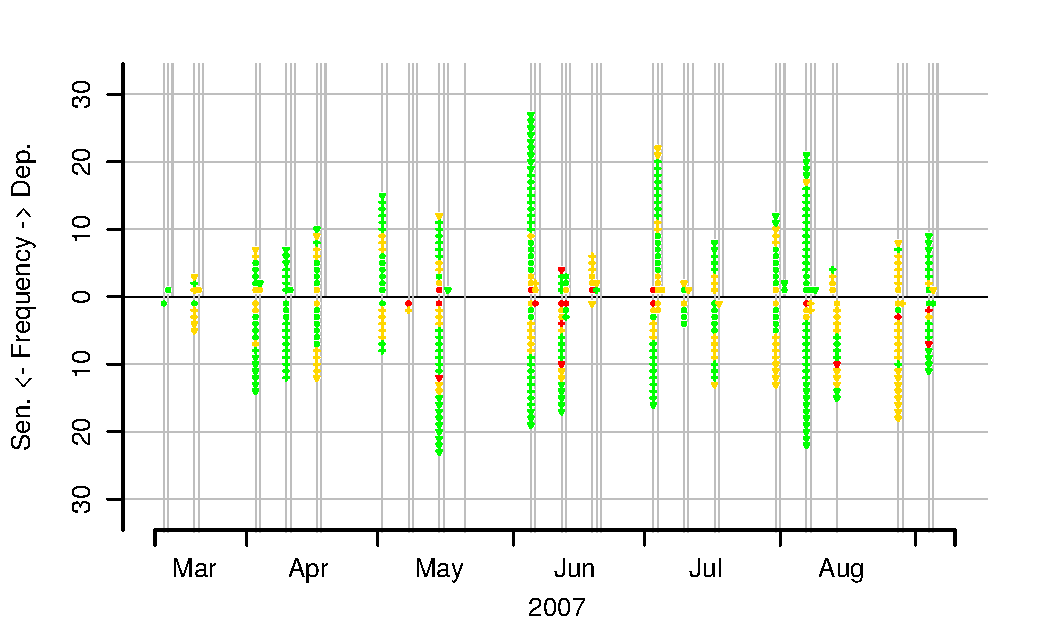
\includegraphics[width=\columnwidth]{../../graphs/urgencias2007-1.pdf} \\

    \begin{tikzpicture}[scale=.1]
      \fill[red]          (0,-1   ) circle (.75);
      \node[right] at     (1.25,-1   ) {\scriptsize{Act now}};  
      \fill[yellow]       (20  ,-1  ) circle (.75);
      \node[right] at     (21.25,-1) {\scriptsize{2-week notice}};  
      \fill[green]        (50  ,-1   ) circle (.75);
      \node[right] at     (51.25,-1 ) {\scriptsize{4-week notice}};  
      \draw[red,thick]    (0  ,-4   )  -- (0,-6);
      \draw[red,thick]    (-1 ,-5   ) -- (1,-5);
      \draw[yellow,thick] (2  ,-4   )  -- (2,-6);
      \draw[yellow,thick] (1  ,-5   ) -- (3,-5);
      \draw[green,thick]  (4  ,-4   )  -- (4,-6);
      \draw[green,thick]  (3  ,-5   ) -- (5,-5);
      \node[right] at     (4.5,-5 ) {\scriptsize{Deadline change}};  
      \fill[red]          (39  ,-4   )  -- (41,-4) -- (40,-6);
      \fill[yellow]       (41  ,-4   )  -- (43,-4) -- (42,-6);
      \fill[green]        (43  ,-4   )  -- (45,-4) -- (44,-6);
      \node[right] at     (44.5,-5  ) {\scriptsize{Withdraw}};  
    \end{tikzpicture}
\end{center}
}
%%%%%%%%%%%%%%%%%%%%%%%%%%%%%%%%%%%%%%%%%%%%%%%%%%%%%%%%%%%%%%%%%%%%%%%%%%%%%%%%%%%%%%%%%%%%%%%%
\frame {                      % SLIDE

    \frametitle{Daily messages 2007--08}

\begin{center}
    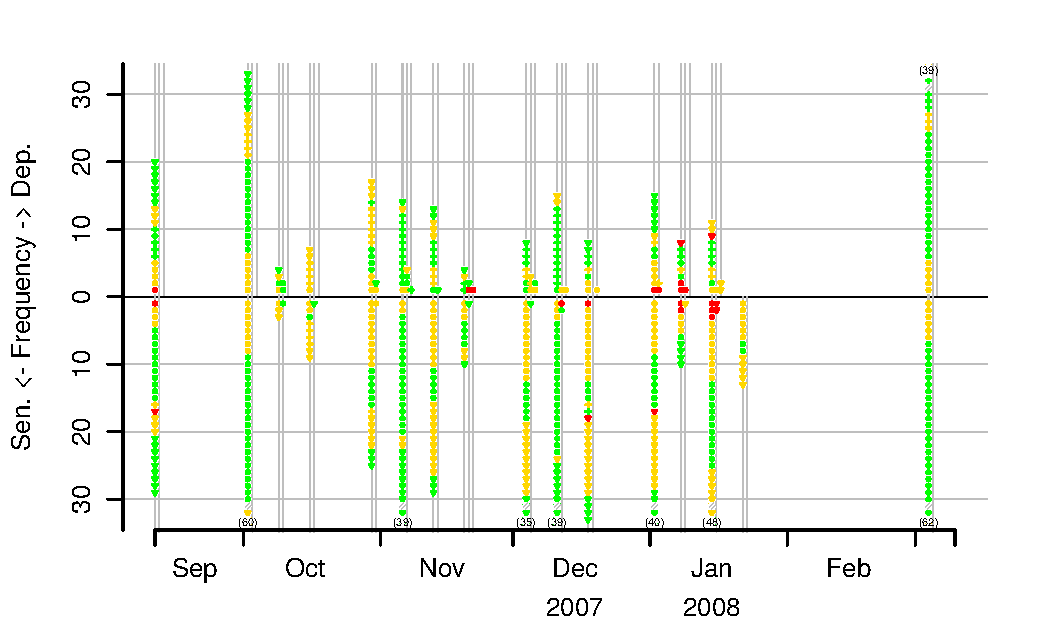
\includegraphics[width=\columnwidth]{../../graphs/urgencias2007-2.pdf} \\

    \begin{tikzpicture}[scale=.1]
      \fill[red]          (0,-1   ) circle (.75);
      \node[right] at     (1.25,-1   ) {\scriptsize{Act now}};  
      \fill[yellow]       (20  ,-1  ) circle (.75);
      \node[right] at     (21.25,-1) {\scriptsize{2-week notice}};  
      \fill[green]        (50  ,-1   ) circle (.75);
      \node[right] at     (51.25,-1 ) {\scriptsize{4-week notice}};  
      \draw[red,thick]    (0  ,-4   )  -- (0,-6);
      \draw[red,thick]    (-1 ,-5   ) -- (1,-5);
      \draw[yellow,thick] (2  ,-4   )  -- (2,-6);
      \draw[yellow,thick] (1  ,-5   ) -- (3,-5);
      \draw[green,thick]  (4  ,-4   )  -- (4,-6);
      \draw[green,thick]  (3  ,-5   ) -- (5,-5);
      \node[right] at     (4.5,-5 ) {\scriptsize{Deadline change}};  
      \fill[red]          (39  ,-4   )  -- (41,-4) -- (40,-6);
      \fill[yellow]       (41  ,-4   )  -- (43,-4) -- (42,-6);
      \fill[green]        (43  ,-4   )  -- (45,-4) -- (44,-6);
      \node[right] at     (44.5,-5  ) {\scriptsize{Withdraw}};  
    \end{tikzpicture}
\end{center}
}
%%%%%%%%%%%%%%%%%%%%%%%%%%%%%%%%%%%%%%%%%%%%%%%%%%%%%%%%%%%%%%%%%%%%%%%%%%%%%%%%%%%%%%%%%%%%%%%%
\frame {                      % SLIDE

    \frametitle{Daily messages 2008--09}

\begin{center}
    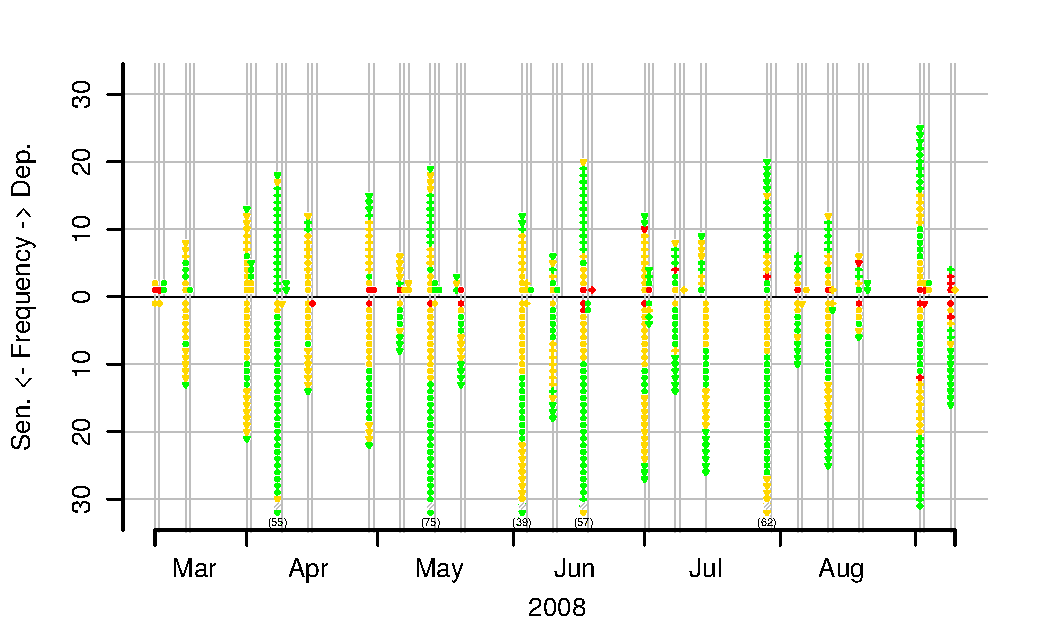
\includegraphics[width=\columnwidth]{../../graphs/urgencias2008-1.pdf} \\

    \begin{tikzpicture}[scale=.1]
      \fill[red]          (0,-1   ) circle (.75);
      \node[right] at     (1.25,-1   ) {\scriptsize{Act now}};  
      \fill[yellow]       (20  ,-1  ) circle (.75);
      \node[right] at     (21.25,-1) {\scriptsize{2-week notice}};  
      \fill[green]        (50  ,-1   ) circle (.75);
      \node[right] at     (51.25,-1 ) {\scriptsize{4-week notice}};  
      \draw[red,thick]    (0  ,-4   )  -- (0,-6);
      \draw[red,thick]    (-1 ,-5   ) -- (1,-5);
      \draw[yellow,thick] (2  ,-4   )  -- (2,-6);
      \draw[yellow,thick] (1  ,-5   ) -- (3,-5);
      \draw[green,thick]  (4  ,-4   )  -- (4,-6);
      \draw[green,thick]  (3  ,-5   ) -- (5,-5);
      \node[right] at     (4.5,-5 ) {\scriptsize{Deadline change}};  
      \fill[red]          (39  ,-4   )  -- (41,-4) -- (40,-6);
      \fill[yellow]       (41  ,-4   )  -- (43,-4) -- (42,-6);
      \fill[green]        (43  ,-4   )  -- (45,-4) -- (44,-6);
      \node[right] at     (44.5,-5  ) {\scriptsize{Withdraw}};  
    \end{tikzpicture}
\end{center}
}
%%%%%%%%%%%%%%%%%%%%%%%%%%%%%%%%%%%%%%%%%%%%%%%%%%%%%%%%%%%%%%%%%%%%%%%%%%%%%%%%%%%%%%%%%%%%%%%%
\frame {                      % SLIDE

    \frametitle{Daily messages 2008--09}

\begin{center}
    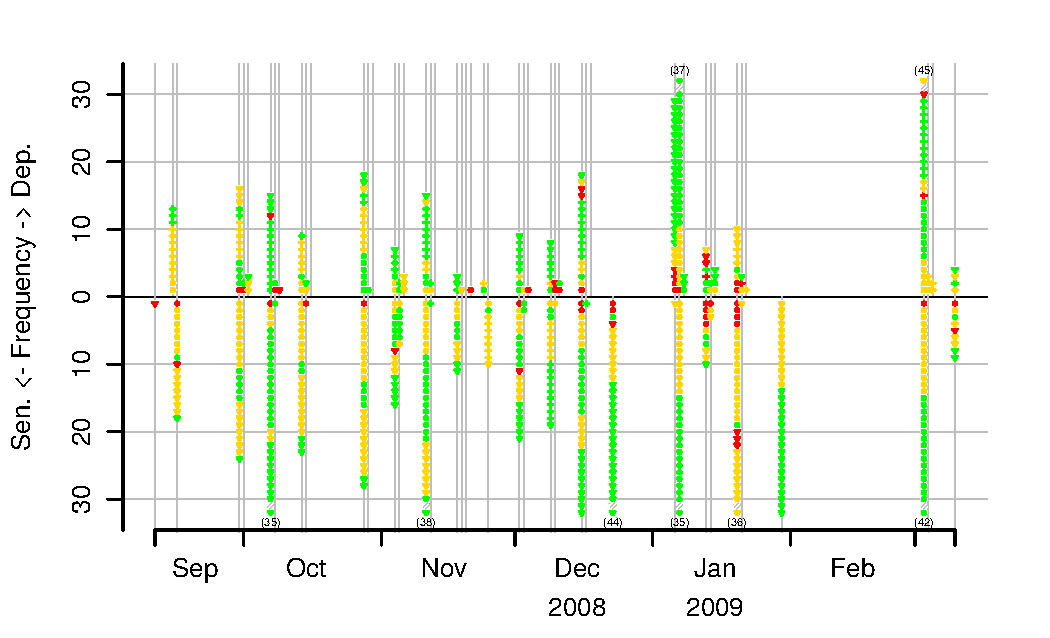
\includegraphics[width=\columnwidth]{../../graphs/urgencias2008-2.pdf} \\

    \begin{tikzpicture}[scale=.1]
      \fill[red]          (0,-1   ) circle (.75);
      \node[right] at     (1.25,-1   ) {\scriptsize{Act now}};  
      \fill[yellow]       (20  ,-1  ) circle (.75);
      \node[right] at     (21.25,-1) {\scriptsize{2-week notice}};  
      \fill[green]        (50  ,-1   ) circle (.75);
      \node[right] at     (51.25,-1 ) {\scriptsize{4-week notice}};  
      \draw[red,thick]    (0  ,-4   )  -- (0,-6);
      \draw[red,thick]    (-1 ,-5   ) -- (1,-5);
      \draw[yellow,thick] (2  ,-4   )  -- (2,-6);
      \draw[yellow,thick] (1  ,-5   ) -- (3,-5);
      \draw[green,thick]  (4  ,-4   )  -- (4,-6);
      \draw[green,thick]  (3  ,-5   ) -- (5,-5);
      \node[right] at     (4.5,-5 ) {\scriptsize{Deadline change}};  
      \fill[red]          (39  ,-4   )  -- (41,-4) -- (40,-6);
      \fill[yellow]       (41  ,-4   )  -- (43,-4) -- (42,-6);
      \fill[green]        (43  ,-4   )  -- (45,-4) -- (44,-6);
      \node[right] at     (44.5,-5  ) {\scriptsize{Withdraw}};  
    \end{tikzpicture}
\end{center}
}
%%%%%%%%%%%%%%%%%%%%%%%%%%%%%%%%%%%%%%%%%%%%%%%%%%%%%%%%%%%%%%%%%%%%%%%%%%%%%%%%%%%%%%%%%%%%%%%%
\frame {                      % SLIDE

    \frametitle{Daily messages 2009--10}

\begin{center}
    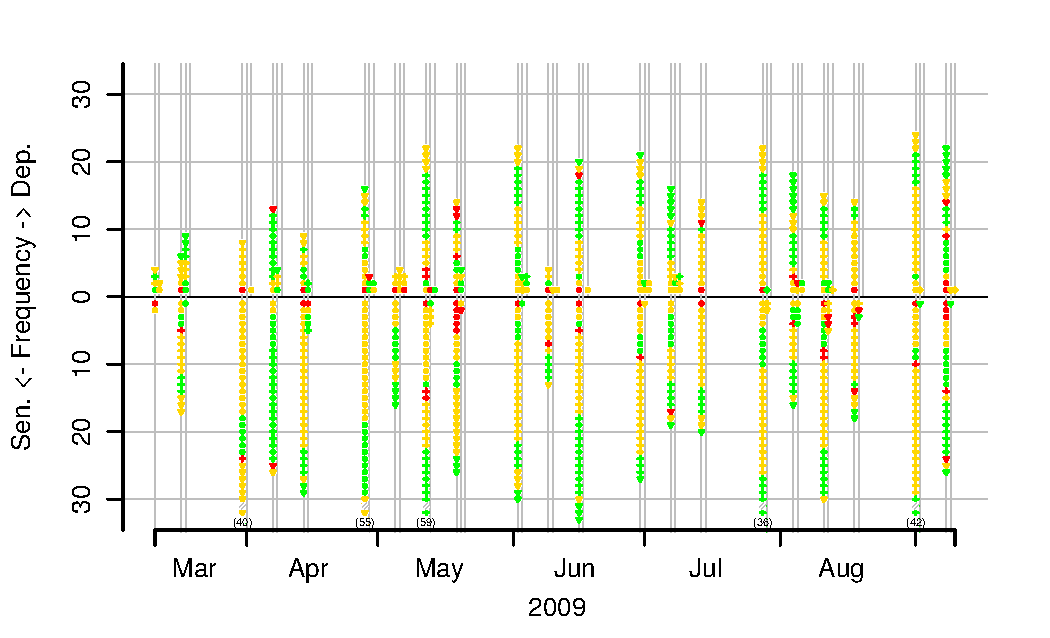
\includegraphics[width=\columnwidth]{../../graphs/urgencias2009-1.pdf} \\

    \begin{tikzpicture}[scale=.1]
      \fill[red]          (0,-1   ) circle (.75);
      \node[right] at     (1.25,-1   ) {\scriptsize{Act now}};  
      \fill[yellow]       (20  ,-1  ) circle (.75);
      \node[right] at     (21.25,-1) {\scriptsize{2-week notice}};  
      \fill[green]        (50  ,-1   ) circle (.75);
      \node[right] at     (51.25,-1 ) {\scriptsize{4-week notice}};  
      \draw[red,thick]    (0  ,-4   )  -- (0,-6);
      \draw[red,thick]    (-1 ,-5   ) -- (1,-5);
      \draw[yellow,thick] (2  ,-4   )  -- (2,-6);
      \draw[yellow,thick] (1  ,-5   ) -- (3,-5);
      \draw[green,thick]  (4  ,-4   )  -- (4,-6);
      \draw[green,thick]  (3  ,-5   ) -- (5,-5);
      \node[right] at     (4.5,-5 ) {\scriptsize{Deadline change}};  
      \fill[red]          (39  ,-4   )  -- (41,-4) -- (40,-6);
      \fill[yellow]       (41  ,-4   )  -- (43,-4) -- (42,-6);
      \fill[green]        (43  ,-4   )  -- (45,-4) -- (44,-6);
      \node[right] at     (44.5,-5  ) {\scriptsize{Withdraw}};  
    \end{tikzpicture}
\end{center}
}
%%%%%%%%%%%%%%%%%%%%%%%%%%%%%%%%%%%%%%%%%%%%%%%%%%%%%%%%%%%%%%%%%%%%%%%%%%%%%%%%%%%%%%%%%%%%%%%%
\frame {                      % SLIDE

    \frametitle{Daily messages 2009--10}

\begin{center}
    \includegraphics[width=\columnwidth]{../../graphs/urgencias2009-2.pdf} \\

    \begin{tikzpicture}[scale=.1]
      \fill[red]          (0,-1   ) circle (.75);
      \node[right] at     (1.25,-1   ) {\scriptsize{Act now}};  
      \fill[yellow]       (20  ,-1  ) circle (.75);
      \node[right] at     (21.25,-1) {\scriptsize{2-week notice}};  
      \fill[green]        (50  ,-1   ) circle (.75);
      \node[right] at     (51.25,-1 ) {\scriptsize{4-week notice}};  
      \draw[red,thick]    (0  ,-4   )  -- (0,-6);
      \draw[red,thick]    (-1 ,-5   ) -- (1,-5);
      \draw[yellow,thick] (2  ,-4   )  -- (2,-6);
      \draw[yellow,thick] (1  ,-5   ) -- (3,-5);
      \draw[green,thick]  (4  ,-4   )  -- (4,-6);
      \draw[green,thick]  (3  ,-5   ) -- (5,-5);
      \node[right] at     (4.5,-5 ) {\scriptsize{Deadline change}};  
      \fill[red]          (39  ,-4   )  -- (41,-4) -- (40,-6);
      \fill[yellow]       (41  ,-4   )  -- (43,-4) -- (42,-6);
      \fill[green]        (43  ,-4   )  -- (45,-4) -- (44,-6);
      \node[right] at     (44.5,-5  ) {\scriptsize{Withdraw}};  
    \end{tikzpicture}
\end{center}
}
%%%%%%%%%%%%%%%%%%%%%%%%%%%%%%%%%%%%%%%%%%%%%%%%%%%%%%%%%%%%%%%%%%%%%%%%%%%%%%%%%%%%%%%%%%%%%%%%
\frame {                      % SLIDE

    \frametitle{Daily messages 2010--11}

\begin{center}
    \includegraphics[width=\columnwidth]{../../graphs/urgencias2010-1.pdf} \\

    \begin{tikzpicture}[scale=.1]
      \fill[red]          (0,-1   ) circle (.75);
      \node[right] at     (1.25,-1   ) {\scriptsize{Act now}};  
      \fill[yellow]       (20  ,-1  ) circle (.75);
      \node[right] at     (21.25,-1) {\scriptsize{2-week notice}};  
      \fill[green]        (50  ,-1   ) circle (.75);
      \node[right] at     (51.25,-1 ) {\scriptsize{4-week notice}};  
      \draw[red,thick]    (0  ,-4   )  -- (0,-6);
      \draw[red,thick]    (-1 ,-5   ) -- (1,-5);
      \draw[yellow,thick] (2  ,-4   )  -- (2,-6);
      \draw[yellow,thick] (1  ,-5   ) -- (3,-5);
      \draw[green,thick]  (4  ,-4   )  -- (4,-6);
      \draw[green,thick]  (3  ,-5   ) -- (5,-5);
      \node[right] at     (4.5,-5 ) {\scriptsize{Deadline change}};  
      \fill[red]          (39  ,-4   )  -- (41,-4) -- (40,-6);
      \fill[yellow]       (41  ,-4   )  -- (43,-4) -- (42,-6);
      \fill[green]        (43  ,-4   )  -- (45,-4) -- (44,-6);
      \node[right] at     (44.5,-5  ) {\scriptsize{Withdraw}};  
    \end{tikzpicture}
\end{center}
}
%%%%%%%%%%%%%%%%%%%%%%%%%%%%%%%%%%%%%%%%%%%%%%%%%%%%%%%%%%%%%%%%%%%%%%%%%%%%%%%%%%%%%%%%%%%%%%%%
\frame {                      % SLIDE

    \frametitle{Daily messages 2010--11}

\begin{center}
    \includegraphics[width=\columnwidth]{../../graphs/urgencias2010-2.pdf} \\

    \begin{tikzpicture}[scale=.1]
      \fill[red]          (0,-1   ) circle (.75);
      \node[right] at     (1.25,-1   ) {\scriptsize{Act now}};  
      \fill[yellow]       (20  ,-1  ) circle (.75);
      \node[right] at     (21.25,-1) {\scriptsize{2-week notice}};  
      \fill[green]        (50  ,-1   ) circle (.75);
      \node[right] at     (51.25,-1 ) {\scriptsize{4-week notice}};  
      \draw[red,thick]    (0  ,-4   )  -- (0,-6);
      \draw[red,thick]    (-1 ,-5   ) -- (1,-5);
      \draw[yellow,thick] (2  ,-4   )  -- (2,-6);
      \draw[yellow,thick] (1  ,-5   ) -- (3,-5);
      \draw[green,thick]  (4  ,-4   )  -- (4,-6);
      \draw[green,thick]  (3  ,-5   ) -- (5,-5);
      \node[right] at     (4.5,-5 ) {\scriptsize{Deadline change}};  
      \fill[red]          (39  ,-4   )  -- (41,-4) -- (40,-6);
      \fill[yellow]       (41  ,-4   )  -- (43,-4) -- (42,-6);
      \fill[green]        (43  ,-4   )  -- (45,-4) -- (44,-6);
      \node[right] at     (44.5,-5  ) {\scriptsize{Withdraw}};  
    \end{tikzpicture}
\end{center}
}
%%%%%%%%%%%%%%%%%%%%%%%%%%%%%%%%%%%%%%%%%%%%%%%%%%%%%%%%%%%%%%%%%%%%%%%%%%%%%%%%%%%%%%%%%%%%%%%%
\frame {                      % SLIDE

    \frametitle{Daily messages 2011--12}

\begin{center}
    \includegraphics[width=\columnwidth]{../../graphs/urgencias2011-1.pdf} \\

    \begin{tikzpicture}[scale=.1]
      \fill[red]          (0,-1   ) circle (.75);
      \node[right] at     (1.25,-1   ) {\scriptsize{Act now}};  
      \fill[yellow]       (20  ,-1  ) circle (.75);
      \node[right] at     (21.25,-1) {\scriptsize{2-week notice}};  
      \fill[green]        (50  ,-1   ) circle (.75);
      \node[right] at     (51.25,-1 ) {\scriptsize{4-week notice}};  
      \draw[red,thick]    (0  ,-4   )  -- (0,-6);
      \draw[red,thick]    (-1 ,-5   ) -- (1,-5);
      \draw[yellow,thick] (2  ,-4   )  -- (2,-6);
      \draw[yellow,thick] (1  ,-5   ) -- (3,-5);
      \draw[green,thick]  (4  ,-4   )  -- (4,-6);
      \draw[green,thick]  (3  ,-5   ) -- (5,-5);
      \node[right] at     (4.5,-5 ) {\scriptsize{Deadline change}};  
      \fill[red]          (39  ,-4   )  -- (41,-4) -- (40,-6);
      \fill[yellow]       (41  ,-4   )  -- (43,-4) -- (42,-6);
      \fill[green]        (43  ,-4   )  -- (45,-4) -- (44,-6);
      \node[right] at     (44.5,-5  ) {\scriptsize{Withdraw}};  
    \end{tikzpicture}
\end{center}
}
%%%%%%%%%%%%%%%%%%%%%%%%%%%%%%%%%%%%%%%%%%%%%%%%%%%%%%%%%%%%%%%%%%%%%%%%%%%%%%%%%%%%%%%%%%%%%%%%
\frame {                      % SLIDE

    \frametitle{Daily messages 2011--12}

\begin{center}
    \includegraphics[width=\columnwidth]{../../graphs/urgencias2011-2.pdf} \\

    \begin{tikzpicture}[scale=.1]
      \fill[red]          (0,-1   ) circle (.75);
      \node[right] at     (1.25,-1   ) {\scriptsize{Act now}};  
      \fill[yellow]       (20  ,-1  ) circle (.75);
      \node[right] at     (21.25,-1) {\scriptsize{2-week notice}};  
      \fill[green]        (50  ,-1   ) circle (.75);
      \node[right] at     (51.25,-1 ) {\scriptsize{4-week notice}};  
      \draw[red,thick]    (0  ,-4   )  -- (0,-6);
      \draw[red,thick]    (-1 ,-5   ) -- (1,-5);
      \draw[yellow,thick] (2  ,-4   )  -- (2,-6);
      \draw[yellow,thick] (1  ,-5   ) -- (3,-5);
      \draw[green,thick]  (4  ,-4   )  -- (4,-6);
      \draw[green,thick]  (3  ,-5   ) -- (5,-5);
      \node[right] at     (4.5,-5 ) {\scriptsize{Deadline change}};  
      \fill[red]          (39  ,-4   )  -- (41,-4) -- (40,-6);
      \fill[yellow]       (41  ,-4   )  -- (43,-4) -- (42,-6);
      \fill[green]        (43  ,-4   )  -- (45,-4) -- (44,-6);
      \node[right] at     (44.5,-5  ) {\scriptsize{Withdraw}};  
    \end{tikzpicture}
\end{center}
}
%%%%%%%%%%%%%%%%%%%%%%%%%%%%%%%%%%%%%%%%%%%%%%%%%%%%%%%%%%%%%%%%%%%%%%%%%%%%%%%%%%%%%%%%%%%%%%%%
\frame {                      % SLIDE

    \frametitle{Daily messages 2012--13}

\begin{center}
    \includegraphics[width=\columnwidth]{../../graphs/urgencias2012-1.pdf} \\

    \begin{tikzpicture}[scale=.1]
      \fill[red]          (0,-1   ) circle (.75);
      \node[right] at     (1.25,-1   ) {\scriptsize{Act now}};  
      \fill[yellow]       (20  ,-1  ) circle (.75);
      \node[right] at     (21.25,-1) {\scriptsize{2-week notice}};  
      \fill[green]        (50  ,-1   ) circle (.75);
      \node[right] at     (51.25,-1 ) {\scriptsize{4-week notice}};  
      \draw[red,thick]    (0  ,-4   )  -- (0,-6);
      \draw[red,thick]    (-1 ,-5   ) -- (1,-5);
      \draw[yellow,thick] (2  ,-4   )  -- (2,-6);
      \draw[yellow,thick] (1  ,-5   ) -- (3,-5);
      \draw[green,thick]  (4  ,-4   )  -- (4,-6);
      \draw[green,thick]  (3  ,-5   ) -- (5,-5);
      \node[right] at     (4.5,-5 ) {\scriptsize{Deadline change}};  
      \fill[red]          (39  ,-4   )  -- (41,-4) -- (40,-6);
      \fill[yellow]       (41  ,-4   )  -- (43,-4) -- (42,-6);
      \fill[green]        (43  ,-4   )  -- (45,-4) -- (44,-6);
      \node[right] at     (44.5,-5  ) {\scriptsize{Withdraw}};  
    \end{tikzpicture}
\end{center}
}
%%%%%%%%%%%%%%%%%%%%%%%%%%%%%%%%%%%%%%%%%%%%%%%%%%%%%%%%%%%%%%%%%%%%%%%%%%%%%%%%%%%%%%%%%%%%%%%%
\frame {                      % SLIDE

    \frametitle{Daily messages 2012--13}

\begin{center}
    \includegraphics[width=\columnwidth]{../../graphs/urgencias2012-2.pdf} \\

    \begin{tikzpicture}[scale=.1]
      \fill[red]          (0,-1   ) circle (.75);
      \node[right] at     (1.25,-1   ) {\scriptsize{Act now}};  
      \fill[yellow]       (20  ,-1  ) circle (.75);
      \node[right] at     (21.25,-1) {\scriptsize{2-week notice}};  
      \fill[green]        (50  ,-1   ) circle (.75);
      \node[right] at     (51.25,-1 ) {\scriptsize{4-week notice}};  
      \draw[red,thick]    (0  ,-4   )  -- (0,-6);
      \draw[red,thick]    (-1 ,-5   ) -- (1,-5);
      \draw[yellow,thick] (2  ,-4   )  -- (2,-6);
      \draw[yellow,thick] (1  ,-5   ) -- (3,-5);
      \draw[green,thick]  (4  ,-4   )  -- (4,-6);
      \draw[green,thick]  (3  ,-5   ) -- (5,-5);
      \node[right] at     (4.5,-5 ) {\scriptsize{Deadline change}};  
      \fill[red]          (39  ,-4   )  -- (41,-4) -- (40,-6);
      \fill[yellow]       (41  ,-4   )  -- (43,-4) -- (42,-6);
      \fill[green]        (43  ,-4   )  -- (45,-4) -- (44,-6);
      \node[right] at     (44.5,-5  ) {\scriptsize{Withdraw}};  
    \end{tikzpicture}
\end{center}
}
%%%%%%%%%%%%%%%%%%%%%%%%%%%%%%%%%%%%%%%%%%%%%%%%%%%%%%%%%%%%%%%%%%%%%%%%%%%%%%%%%%%%%%%%%%%%%%%%
\frame {                      % SLIDE

    \frametitle{Daily messages 2013--14}

\begin{center}
    \includegraphics[width=\columnwidth]{../../graphs/urgencias2013-1.pdf} \\

    \begin{tikzpicture}[scale=.1]
      \fill[red]          (0,-1   ) circle (.75);
      \node[right] at     (1.25,-1   ) {\scriptsize{Act now}};  
      \fill[yellow]       (20  ,-1  ) circle (.75);
      \node[right] at     (21.25,-1) {\scriptsize{2-week notice}};  
      \fill[green]        (50  ,-1   ) circle (.75);
      \node[right] at     (51.25,-1 ) {\scriptsize{4-week notice}};  
      \draw[red,thick]    (0  ,-4   )  -- (0,-6);
      \draw[red,thick]    (-1 ,-5   ) -- (1,-5);
      \draw[yellow,thick] (2  ,-4   )  -- (2,-6);
      \draw[yellow,thick] (1  ,-5   ) -- (3,-5);
      \draw[green,thick]  (4  ,-4   )  -- (4,-6);
      \draw[green,thick]  (3  ,-5   ) -- (5,-5);
      \node[right] at     (4.5,-5 ) {\scriptsize{Deadline change}};  
      \fill[red]          (39  ,-4   )  -- (41,-4) -- (40,-6);
      \fill[yellow]       (41  ,-4   )  -- (43,-4) -- (42,-6);
      \fill[green]        (43  ,-4   )  -- (45,-4) -- (44,-6);
      \node[right] at     (44.5,-5  ) {\scriptsize{Withdraw}};  
    \end{tikzpicture}
\end{center}
}
%%%%%%%%%%%%%%%%%%%%%%%%%%%%%%%%%%%%%%%%%%%%%%%%%%%%%%%%%%%%%%%%%%%%%%%%%%%%%%%%%%%%%%%%%%%%%%%%
\frame {                      % SLIDE

    \frametitle{Daily messages 2013--14}

\begin{center}
    \includegraphics[width=\columnwidth]{../../graphs/urgencias2013-2.pdf} \\

    \begin{tikzpicture}[scale=.1]
      \fill[red]          (0,-1   ) circle (.75);
      \node[right] at     (1.25,-1   ) {\scriptsize{Act now}};  
      \fill[yellow]       (20  ,-1  ) circle (.75);
      \node[right] at     (21.25,-1) {\scriptsize{2-week notice}};  
      \fill[green]        (50  ,-1   ) circle (.75);
      \node[right] at     (51.25,-1 ) {\scriptsize{4-week notice}};  
      \draw[red,thick]    (0  ,-4   )  -- (0,-6);
      \draw[red,thick]    (-1 ,-5   ) -- (1,-5);
      \draw[yellow,thick] (2  ,-4   )  -- (2,-6);
      \draw[yellow,thick] (1  ,-5   ) -- (3,-5);
      \draw[green,thick]  (4  ,-4   )  -- (4,-6);
      \draw[green,thick]  (3  ,-5   ) -- (5,-5);
      \node[right] at     (4.5,-5 ) {\scriptsize{Deadline change}};  
      \fill[red]          (39  ,-4   )  -- (41,-4) -- (40,-6);
      \fill[yellow]       (41  ,-4   )  -- (43,-4) -- (42,-6);
      \fill[green]        (43  ,-4   )  -- (45,-4) -- (44,-6);
      \node[right] at     (44.5,-5  ) {\scriptsize{Withdraw}};  
    \end{tikzpicture}
\end{center}
}


%%%%%%%%%%%%%%%%%%%%%%%%%%%%%%%%%%%%%%%%%%%%%%%%%%%%%%%%%%%%%%%%%%%%%%%%%%%%%%%%%%%%%%%%%%%%%%%%
%%%%%%%%%%%%%%%%%%%%%%%%%%%%%%%%%%%%%%%%%%%%%%%%%%%%%%%%%%%%%%%%%%%%%%%%%%%%%%%%%%%%%%%%%%%%%%%%
%%%%%%%%%%%%%%%%%%%%
%%%%%%%%%%%%%%%%%%%%
%%%%%%%%%%%%%%%%%%%%
\end{document}
%%%%%%%%%%%%%%%%%%%%
%%%%%%%%%%%%%%%%%%%%
%%%%%%%%%%%%%%%%%%%%
%%%%%%%%%%%%%%%%%%%%%%%%%%%%%%%%%%%%%%%%%%%%%%%%%%%%%%%%%%%%%%%%%%%%%%%%%%%%%%%%%%%%%%%%%%%%%%%%
%%%%%%%%%%%%%%%%%%%%%%%%%%%%%%%%%%%%%%%%%%%%%%%%%%%%%%%%%%%%%%%%%%%%%%%%%%%%%%%%%%%%%%%%%%%%%%%%
